% !TeX root = ../main.tex

\chapter{模型自适应的高效压缩方法}

\section{引言}

近年来,深度学习快速发展,已在许多任务中达到了优异的性能表现,使其越来越多的应用在众多生活与工业领域。但这些深度神经网络模型优异的性能都依赖于具有数百万甚至数十亿个参数的深度网络模型,需要消耗大量的计算资源和存储资源,需要高性能的硬件作为支撑,这对实际部署、运行和应用的环境提出了较高的要求。因此,深度神经网络的压缩与优化一直都是一个非常关键的问题,特别是对于计算资源有限的嵌入式移动设备来说,如此高的计算资源要求是不可接受的。另一个关键的挑战是能源消耗:由于移动设备的电池有限,繁重的计算会很快耗尽电池。然而大多数的模型压缩算法与高效的网络结构对于计算硬件并不友好,虽然能够显著模型参数,但是并没有很好的利用硬件性能,达到理论的上的加速比。

在任意深度学习的应用场景落地一个模型/算法时,需要经历两个基本步骤:
\section{动机实验}
\subsection{存储压缩与训练耗时}
\label{m1}
表\ref{KD}展示了一个简单CNN网络在cifar10数据集上的训练表现,该结果从训练时长和压缩模型体积的有效性两个角度论证了现有知识蒸馏方法的优点和缺点。从其压缩模型体积的有效性的角度来讲,在使用了知识蒸馏的训练方法后,一个使用常规训练5层CNN网络的图片分类精度还略低于使用了知识蒸馏的3层CNN网络,前者是0.791\%后者是0.804\%。在相同精度的约束条件下,仅使用3层CNN网络就能达到5层CNN网络的图片分类效果,但是其存储体积却远远小于5层CNN网络。表\ref{KD}中统计的是模型压缩文件,即格式为\emph{.pth.tar}的文件,这类文件格式是常规模型文件\emph{.pth}的无损压缩版本,压缩版本的模型存储文件格式并不会对模型精度造成损失。同等精度条件下,3层CNN网络的静态数据仅需要1.32MB的存储空间开销,而5层CNN网络却需要4.11MB的存储空间开销,后者的开销是前者的3.11倍。这说明了知识蒸馏是压缩卷积神经网络模型的有力工具,能够让小尺寸模型达到和大尺寸模型相同的精度表现。
\begin{table}[]
	\begin{tabular}{lcccc}
		\hline
		\caption{在\emph{Cifar10}数据集上,以学习率=0.01,蒸馏温度=20,alpha=0.9,批大小=128,adam优化器,30个epoch的训练结果。其中 “单独训练” 指仅使用网络本身进行常规的训练,“知识蒸馏” 指采用了验证精度为0.945\%的教师网络Resnet18的训练结果,“模型尺寸” 统计的是模型压缩文件\emph{.pth.tar}的总大小。}
		\label{KD}
		& \begin{tabular}[c]{@{}c@{}}\textbf{训练时间}\\(s)\end{tabular} & \begin{tabular}[c]{@{}c@{}}\textbf{额外FLOPs}\\(B)\end{tabular} & \begin{tabular}[c]{@{}c@{}}\textbf{准确率}\\(\%)\end{tabular} & \begin{tabular}[c]{@{}c@{}}\textbf{模型尺寸}\\ (MB)\end{tabular} \\    \hline
		5层网络    &\multirow{2}{*}{207}  &\multirow{2}{*}{/}           & \multirow{2}{*}{\textbf{0.791}}  & \multirow{2}{*}{\textbf{4.11}}         \\ 
		(单独训练) &     &             &                  &                \\ \hline
		
		5层网络    &\multirow{2}{*}{\textbf{273}}  &\multirow{2}{*}{33399.32}           & \multirow{2}{*}{0.843}  & \multirow{2}{*}{4.11}         \\ 
        (知识蒸馏) &     &             &                  &                \\ \hline		
		
		3层网络    &\multirow{2}{*}{\textbf{269}}  &\multirow{2}{*}{33399.32}           & \multirow{2}{*}{\textbf{0.804}}  & \multirow{2}{*}{\textbf{1.32}}         \\ 
		(知识蒸馏) &     &             &                  &                \\ \hline
	\end{tabular}
\end{table}

但是,从训练时长的角度来讲,虽然使用了知识蒸馏之后,模型的精度明显得到提升,但却要耗费比常规训练1.29-1.31倍的训练时长开销。表\ref{KD}所示,使用了知识蒸馏方法的第二行和第三行的训练时长明显多于常规训练的第一行。出现这样现象的原因是因为在知识蒸馏过程中,一张图片需要教师网络推理一次后,学生网络再推理一次,这使得知识蒸馏在训练过程中除了学生网络的反向梯度更新之外,还需要花费算力在教师网络的推理中。在本次实验设置中,约多花费了33399.32B次浮点运算总数。值得注意的是,5层CNN网络和3层CNN网络的知识蒸馏耗时却相差不明显,它们的训练耗时分别是273秒和269秒。这说明了在知识蒸馏过程中,大量的时间被花费在了教师网络的前向推理上。并且,随着教师网络尺寸的增大,该耗时占比还会进一步提升。

\subsection{蒸馏精度与教师网络尺寸}
\label{m2}
虽然知识蒸馏的训练方式,能够有效地将大尺寸网络的知识注入到小尺寸的网络中,从而明显地压缩模型存储空间开销。但是,模型的压缩比率是存在上限的,即教师网络和学生网络之间的尺寸差距若过大,那么反倒会出现模型精度的损失下降,这即是\textbf{capacity gap}\cite{gou2021knowledge,guo2020reducing}问题。表 \ref{gap}展示了学生网络resnet18使用知识蒸馏在imagnenet数据集上的训练结果。可以看到resnet50图片分类误差是23.85\%,在所有三个网络中是最低的。但是,用其作为resnet18的教师网络进行知识蒸馏,其图片分类误差反倒出现了上升。对比于,resnet34做教师网络教学resnet18,resnet50的教学效果反倒让图片分类误差上升了0.16\%。表中第四列展示了,随着网络尺寸的增加,学生网络resnet18的图片分类误差反倒出现逐渐上升的趋势,图片分类误差最多达到了0.71\%的增幅。出现这样的结果的原因在于,在训练小尺寸模型时,强迫学生模仿教师的过拟合结果会损害学生的精度表现。即,并不是越大的网络就一定能训练出符合精度要求的小尺寸紧凑模型。除此之外,结合表\ref{KD}的实验结论,在知识蒸馏训练紧凑模型的过程中,教师网络的前向推理时间会消耗大量训练时长。选择越大的网络会明显增多训练耗时,并且,不一定就能够提高模型压缩比率,反倒还会出现下降。
\begin{table}[]
	\begin{tabular}{cccc}

		\hline
		\caption{教师网络与学生网络的capacity gap\cite{gou2021knowledge,guo2020reducing}问题。在\emph{Imagnet}数据集上,以学习率=0.01,蒸馏温度=20,alpha=0.9,批大小=256,动量系数=0.9的标准SGD优化器,200个epoch的训练结果\cite{cho2019efficacy}。}
		\label{gap}
		\textbf{教师网络} &\textbf{教师网络误差(\%)} &\textbf{学生网络误差(\%)}   &\textbf{误差上升(\%)}\\ \hline
		/                          & /                               & 30.24    & /                       \\ 
		Resnet18                   & 30.24                           & 30.57    & 0.33                      \\ 
		Resnet34                   & 26.7                            & 30.79    & 0.55                      \\ 
		Resnet50                   & 23.85                           & 30.95    & 0.71                \\ \hline
	\end{tabular}
\end{table}

上述动机实验表明,既然尺寸越大的教师网络,并不一定就能提升压缩比例和蒸馏精度。选用过大尺寸的教师网络反倒还会增加训练时长。因此,为了进一步探究蒸馏精度与网络尺寸之间的关系,本文在cifar10数据集上进一步实验,采用较小网络和大网络轮番教学的方式探究教师网络模型尺寸对精度的影响。图\ref{kd_cmp}展示了一个五层CNN在cifar上的实验结果。图\ref{kd_cmp_first}中在前15个epoch中使用resnet18教学紧凑网络,而在后15个epoch切换至resnet50教学学生网络。结果表明在前期使用resnet18,后期使用resnet50进行蒸馏的方案的蒸馏精度对比于全程使用resnet50的方案在验证集上的精度仅低了0.005\%,前者为0.837\%,后者为0.842\%,但是训练速度却快了1.4倍。出现这样的提速是因为前15个epoch采用resnet18进行推理,其一次前向推理耗时显著低于resnet50耗时。该实验证明了,在知识蒸馏过程中,前期采用小尺寸网络进行教学并不影响最终精度表现,并能够显著减少训练时长。

\begin{figure*}[h]
	\centering
	\subfigure[在第15个epoch切换主教师网络的训练结果]{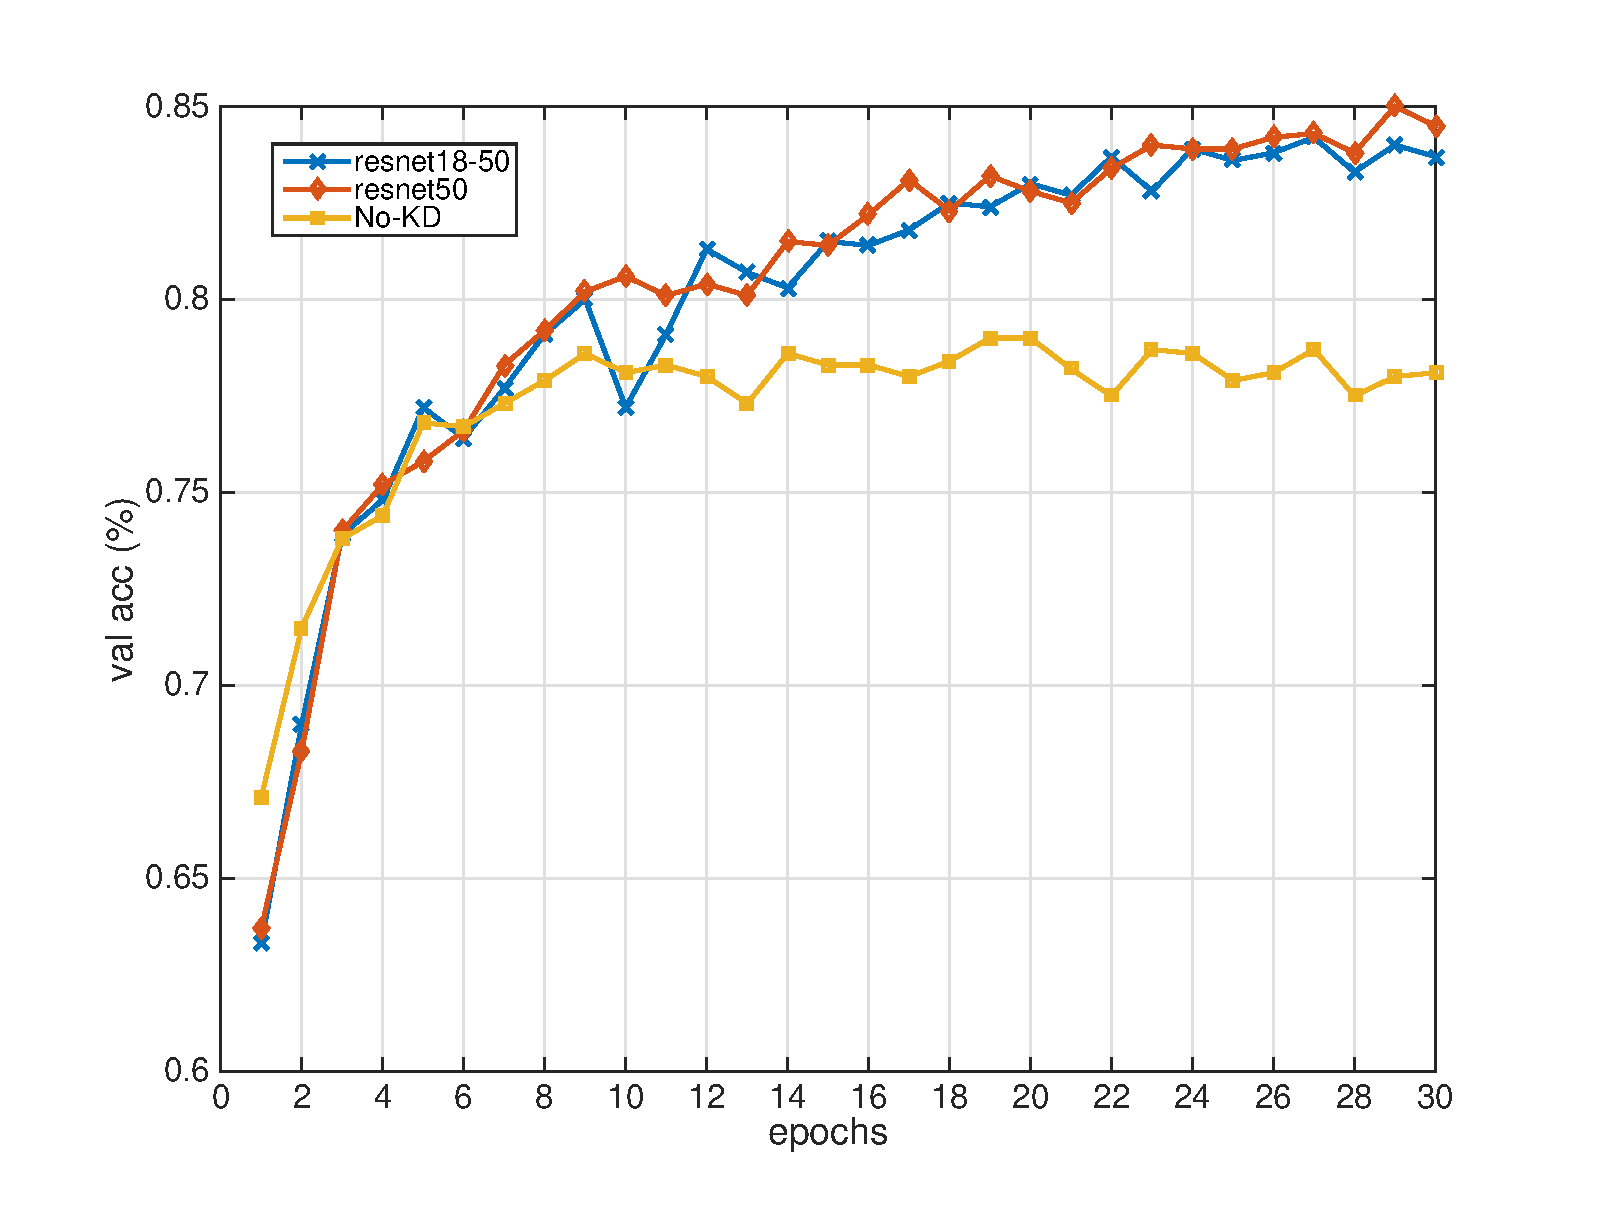
\includegraphics[width=0.9\textwidth]{figures/15_inter_distill.eps}
		\label{kd_cmp_first}}
	\subfigure[在第9个epoch切换主教师网络的训练结果]{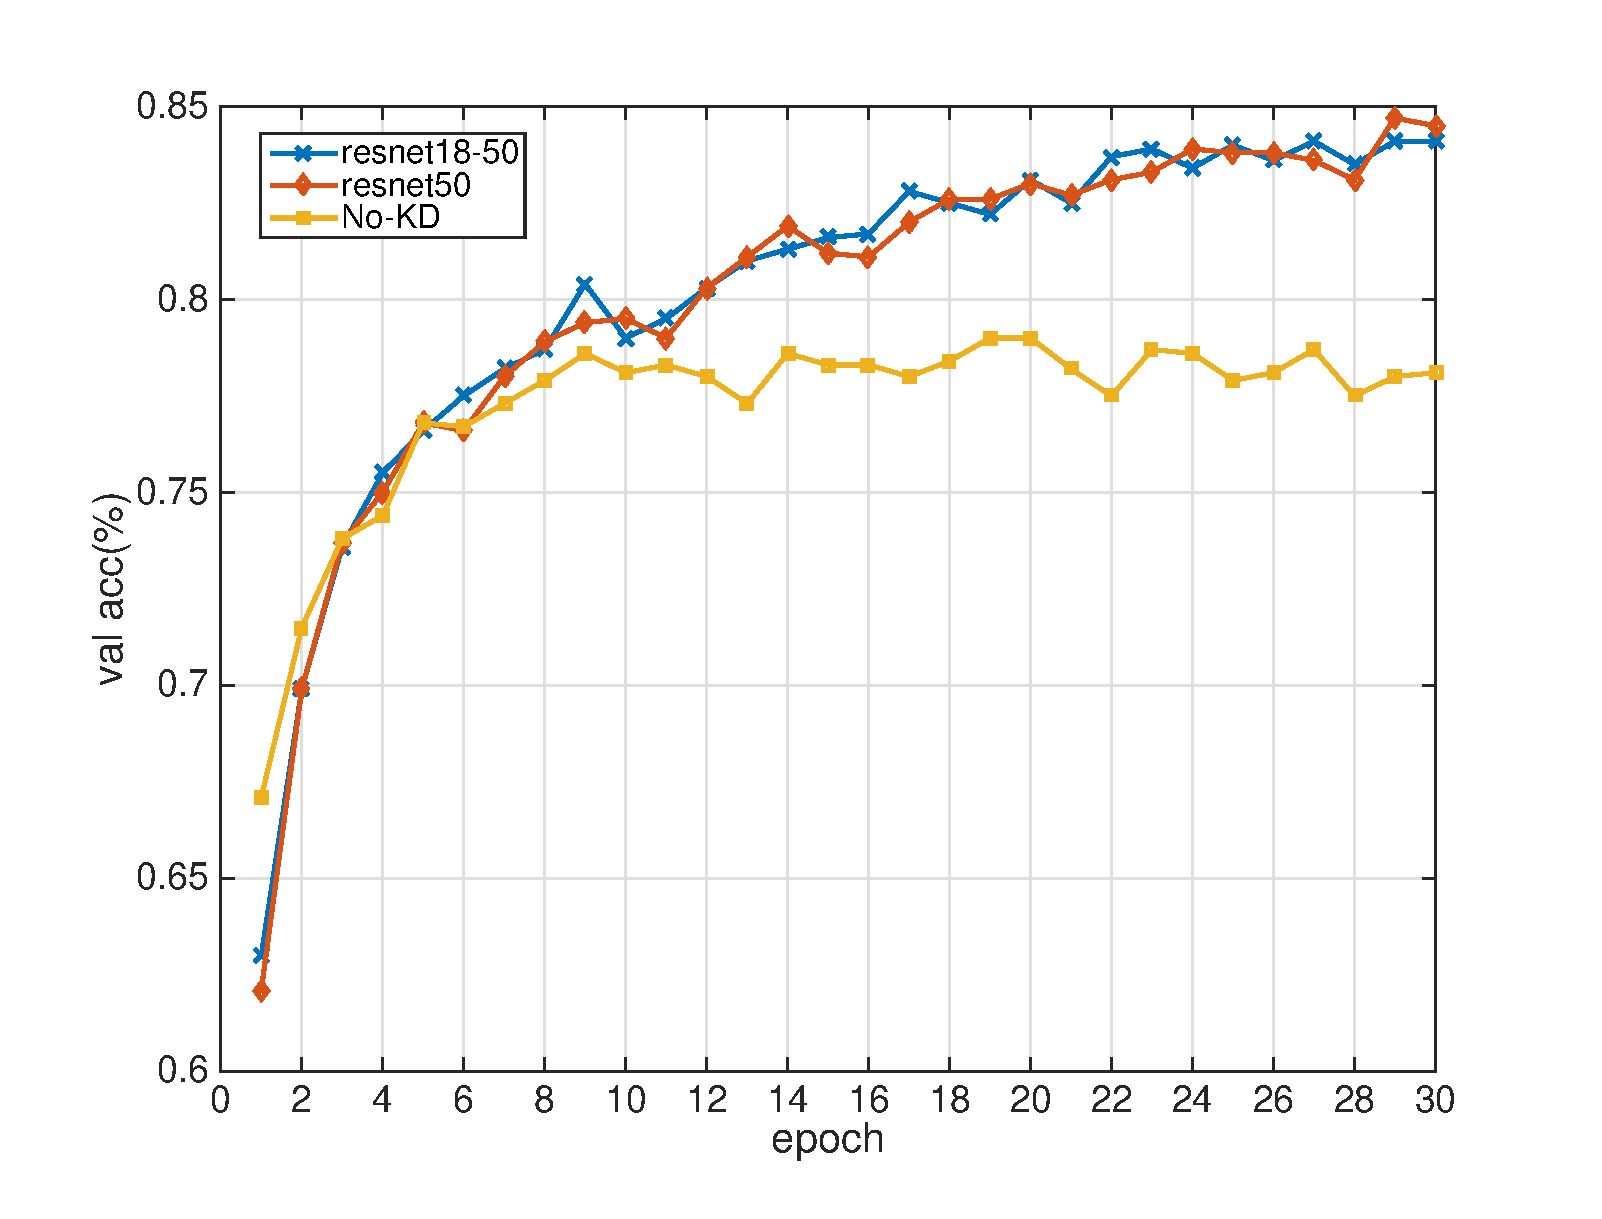
\includegraphics[width=0.9\textwidth]{figures/9_inter_distill.eps}
		\label{kd_cmp_second}}
	\caption{在\emph{Cifar10}数据集上,以学习率=0.01,批大小=128,蒸馏温度=20,alpha=0.9,adam优化器,30个epoch的训练结果其中 \emph{resnet18-50}指采用两个教师网络教学,辅助网络为resnet18,主教师网络为resent50。 \emph{resnet50} 指采用教师教师网络为resnet50的常规知识蒸馏方法。 \emph{No-Kd} 指不使用知识蒸馏的常规训练方式。}
	\label{kd_cmp}
\end{figure*}


值得注意的是,在图\ref{kd_cmp_first}中的第10个epoch中,五层紧凑CNN网络的验证精度出现了一个明显的下滑。本文推测,这是因为五层紧凑CNN网络已经无法从resnet18中学习到更多额外知识,因此出现一个明显的精度下滑。为了进行实验对比,图\ref{kd_cmp_second}实验中将教学切换时机更改为在第9个epoch处。实验结果表明,在这样的参数设置下,与全程使用resnet50教学的知识蒸馏方案之间的精度差距进一步缩小至0.001\%,优于在第15个epoch处切换。这说明在知识蒸馏过程不断迭代时,学生网络的学习能力也在不断变强。知识蒸馏整个过程需要动态调整教学策略,以更好的教学学生网络,以进一步提升压缩比率。

综合\ref{m1}和\ref{m2}的内容,我们可以得到如下结论:
\begin{itemize}
	%\vspace{-1em}
	\item 在知识蒸馏训练压缩训练小尺寸紧凑模型时,选用越大的教师网络会显著增多额外浮点操做总次数,从而明显的增多训练耗时;
	\item 当小尺寸紧凑模型和教师网络之间的学习能力差距过于大时,教师网络不仅不会提升训练精度,反倒还会损害模型精度表现;
	\item 知识蒸馏压缩是一个动态的压缩训练过程,紧凑网络的学习能力随着迭代次数的增加而不断提升;
\end{itemize}


\section{自适应高效知识蒸馏压缩方法}
基于上述动机实验观察,我们提出自适应高效知识蒸馏压缩训练小尺寸紧凑模型的方法。我们认为,知识蒸馏压缩训练的过程应该当是自动适应小尺寸紧凑网络模型的学习过程而不断变化的,而不是一直静态的。1) 在知识蒸馏压缩训练的前期阶段,小尺寸紧凑模型与大尺寸网络模型的学习能力差距十分大。2) 在知识蒸馏压缩训练的中后期阶段,随着小尺寸模型不断训练学习,其与大尺寸模型的能力差距逐渐减少。因此,若在知识蒸馏压缩训练的初期,便一直静态采用大尺寸模型教学,不仅会损害模型精度压缩比率,还会显著增加训练耗时。
\subsection{自适应高效知识蒸馏}
\begin{figure}[h]
	\centering
	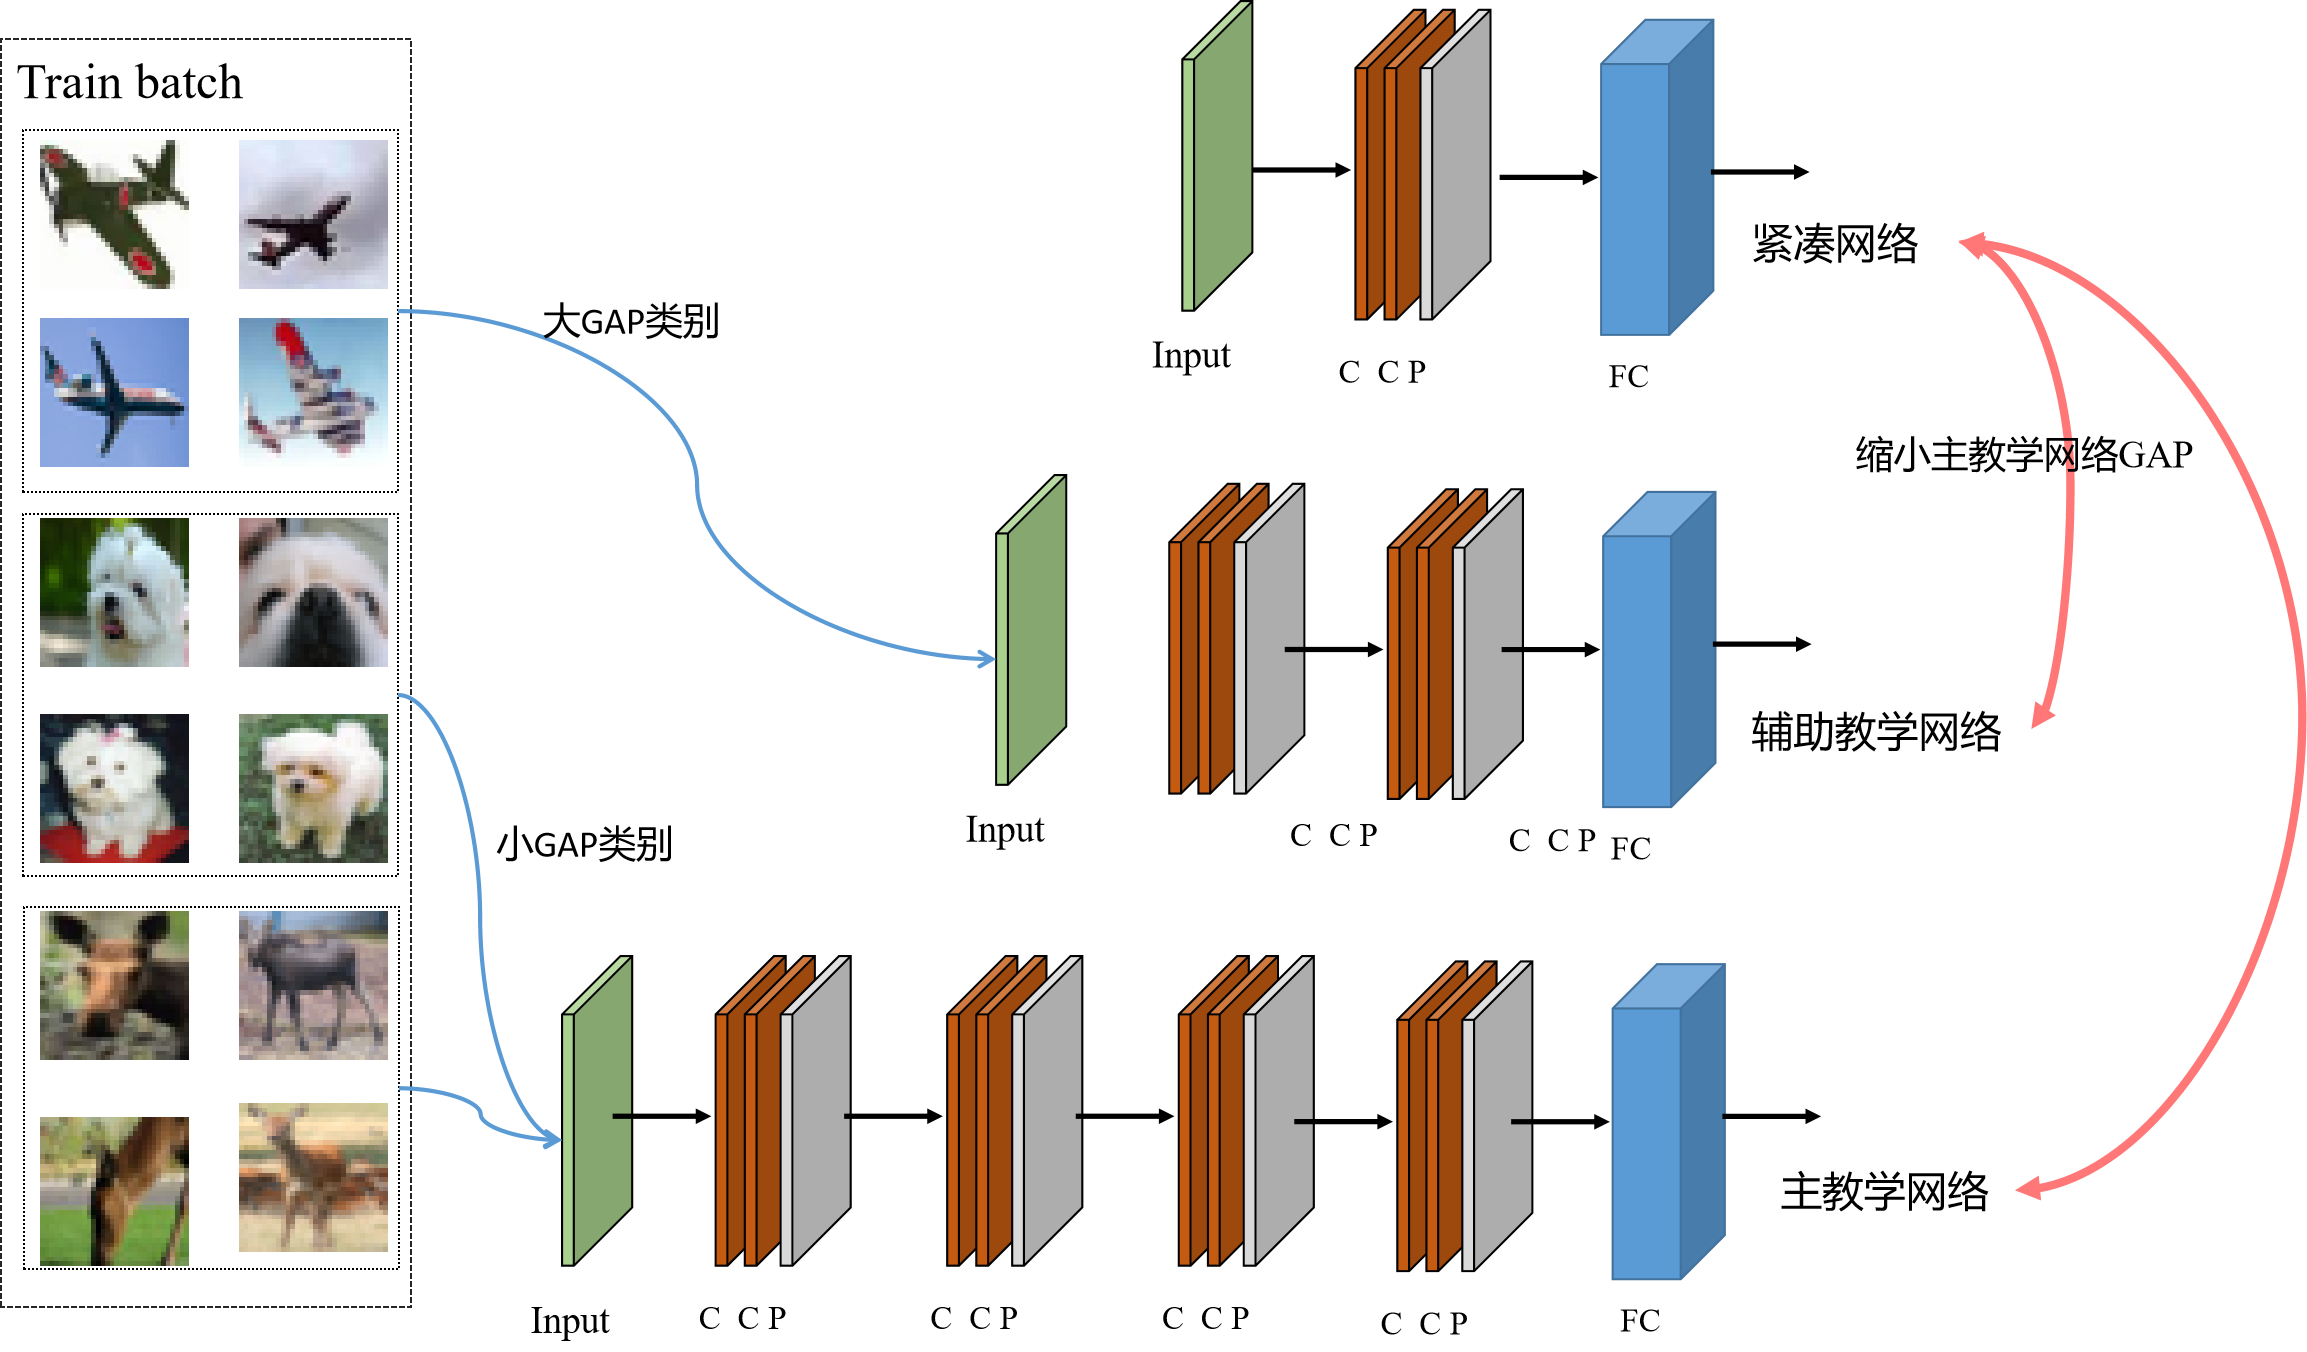
\includegraphics[width=1\textwidth]{figures/adaptive_frame.png}
	\caption{自适应知识蒸馏框架。}
	\label{frame}
\end{figure}
为解决这一问题,我们在小尺寸紧凑模型和大尺寸模型之间引入一个辅助教学网络。该网络尺寸介于小尺寸紧凑网络模型和大尺寸网络模型之间,其主要职责是负责小尺寸紧凑网络模型的前期教学,一旦当小尺寸网络模型和大尺寸网络模型之间的差异缩小到某个可接受范围之内后,便切换至大尺寸网络继续教学。图\ref{frame}展示了完整的自适应蒸馏框架。通过在主教学网络和紧凑网络之间引入辅助教学网络缩小它们之间的差距。在任何一组训练batch中,我们将训练数据分为大gap类别和小gap类别,这样的分类信息来自于上一次epoch。对于大gap类别图像,我们采用辅助教学网络进行教学,用于缩小紧凑网络和主教学网络之间的差距,一旦当差距缩小到可接受范围时,我们便将其归类为小gap类别。小gap类别将采用主教学网络进行精细化教学,用于进一步提升精度。

在知识蒸馏压缩训练刚启动时,数据集中的所有图片都被预先划分到大GAP类别中,随着训练迭代,紧凑网络的学习能力提升,大GAP类别中的部分图片被划入到小GAP类别中,这样便启用主教学网络教学,直至所有图片都被划入到小GAP类别或达到训练迭代次数上限便停止。这样可以明显的提升模型压缩比例和减少整体训练耗时。


\subsection{知识蒸馏方式}
知识蒸馏的核心思想是,教师网络的输出的软标签包含了关于数据点的更多信息,而不仅仅是类标签。例如,如果为一张图像分配了多个类别的高概率,则这可能意味该图像的有极大可能是位于这些类别之间的决策边界附近。因此,强迫让紧凑的学生网络模仿这些可能性能够有效让紧凑的学生网络学习到教师网络在硬标签信息之外发现的一些额外的知识。从而,让有更少参数量的紧凑学生网络依然能够取得和大尺寸网络相当的精度表现。

具体地来说,给定任意一张图片x,在经过教师网络的各层卷积核提取特征后并由全连接层输出一个各类别可能的分数向量 $s(x)$:

\begin{equation}
s(x) = [s_1(x),s_2(x),...,s_K(x)]
\end{equation}

该向量由softamx函数\ref{softmax1},被归一化到0-1区间的最终可能性,分数向量经过softmax函数后输出的向量被称作\textbf{logits}。
\begin{equation}
\begin{aligned}
\label{softmax1}
p(x)_j = \frac{e^{s_j(x)}}{\sum_{k=1}^N e^{s_k(x)}}  (j=1....K)
\end{aligned}
\end{equation}
但是,教学网络的输出\textbf{logits}通常包含了输入图片的最高可能性,这可能会损失部分知识信息,降低紧凑学生网络的精度表现。因此,Hinton等人\cite{hinton2015distilling}提出用\textbf{蒸馏温度}软化教师/学生网络的输出可能性,改造后带温度的softmax函数\ref{softmax2}如下所示。
\begin{equation}
\begin{aligned}
\label{softmax2}
p(x)^{\sim}_j = \frac{e^{s_j(x)}/\tau}{\sum_{k=1}^N e^{s_k(x)/\tau}}  (j=1....K)
\end{aligned}
\end{equation}
其中蒸馏温度$\tau>1$,该参数是一个超参数,需要人为设定。$\tau$值越大,会产生越平滑的概率分布,当$\tau=1$时,就是标准的softmax函数。

紧凑学生网络的用于反向传播优化的loss函数$L$,是典型的交叉熵$L_{cls}$和知识提取$L_{KD}$的线性组合。即,在训练中从数据集中最小化每个图片示例的$L$。
\begin{equation}
\begin{aligned}
\label{loss}
L = \alpha L_{cls} + (1 - \alpha)L_{KD}
\end{aligned}
\end{equation}
其中$L_{KD}$的公式如\ref{lkd}所示:
\begin{equation}
\begin{aligned}
\label{lkd}
L_{KD} = -\alpha \tau^2 \sum_{k}p^{\sim t}_{k}(x)logp^{\sim s}_{k}(x)
\end{aligned}
\end{equation}
公式\ref{loss}中的$\alpha$用于权衡加权两个损失的线性和,是一个超参数,大量实践经验\cite{zagoruyko2016paying,huang2017like,lan2018knowledge,hinton2015distilling}表明当$\alpha=0.9$时,知识蒸馏有着最好的平均性能。公式\ref{lkd}中$p^{\sim t}$指教师网络输出的\emph{logits},$p^{\sim s}$指学生网络输出的\emph{logits}。



\subsection{训练集感知的自适应策略}
随着知识蒸馏训练过程的不停迭代,紧凑学生网络的学习能力逐渐变强。具体地来讲,即是紧凑学生网络对同一个训练组(train batch)图片示例的输出概率分布会逐渐趋近于教师网络。对于紧凑学生网络已经掌握的训练组重复使用辅助网络教学,并不会让紧凑学生网络学习到更多额外的知识,因此一旦当紧凑学生网络对某一个训练组的输出概率分布逼近于辅助教学网络时,便可以切换至有更多额外知识的主教学网络进行教学,提升紧凑学生网络的精度表现。为衡量紧凑学生网络对某一个训练组的学习掌握情况,本文采用非对称距离度量KL散度,用于度量紧凑学生网络和辅助教学网络之间的概率分布间的差异。根据KL散度的信息,对单个训练组动态的选择教学网络。具体地来说,对于单张输入图片x,教师网络与紧凑学生网络之间输出概率分布的KL散度\ref{kl}为:

\begin{equation}
\begin{aligned}
\label{kl}
D_{KL}(p^{t}(x)||p^{s}(x))=\sum_{i=1}^{K}(p^{t}_{k}(x)logp^{t}_{k}(x) - p^{t}_{k}(x)logp^{s}_{k}(x)) (i=1....K)
\end{aligned}
\end{equation}
其中$p^{t}(x)$为教师网络输出概率分布,$p^{s}(x)$为学生网络输出概率分布。对于一个训练组$B$(train batch),教师网络与学生网络之间的输出概率分布KL散度被定义为:
\begin{equation}
\begin{aligned}
\label{kl_batch}
D_{KL}(p^{t}(B)||p^{s}(B))= \frac{\sum_{i=1}^{K}D_{KL}(p^{t}(x_i)||p^{s}(x_i))}{batchsize} (i=1....batchsize)
\end{aligned}
\end{equation}
其中,\emph{batchsize}是当前训练组的尺寸大小。该公式\ref{kl_batch}即表示训练组中所有输入图片x的教师网络与学生网络概率分布KL散度平均值。

使用上述定义到训练组概率分布的KL散度,我们便可以根据紧凑学生网络的输出,进行训练集感知的自适应教师选择。如算法\ref{alm2}所示,其主要流程如下:
\begin{itemize}
	\item 预先加载主教师网络模型和辅助教师网络模型。 
	\item 在每一次训练迭代时,计算学生网络和辅助教师网络模型之间的训练组KL散度值。
	\item 对于KL散度小于可接受阈值$\sigma$的训练组,启用主教师网络模型教学,反之则继续使用辅助教学网络模型。
\end{itemize}

\begin{algorithm}[H]
	\caption{Adaptive knowledge distillation}
	\SetKwFunction{Unio}{Union}
	\SetKwInOut{Input}{input}
	\SetKwInOut{Output}{output}
	
	\Input{A main teacher model with lager size and higher accuracy $T_m$, a assistant teacher model with proper size and acceptable accuracy $T_a$, a lightweight model to be trained $S$, train batch kullback-leibler divergence $KL_{batch}(.)$ defined in Eq.\ref{kl_batch}, distillation loss $Loss(.)$ defined in Eq.\ref{loss}, distillation temperature $\tau$, hyperparameter $\alpha$ and threshold $\sigma$.}
	\Output{lightweight, compressed and high accuracy model $S$.}
	\BlankLine
	
	\For{$i=1,\cdots,epochs$}{
		\For{$j=1,\cdots, \frac{length(dataset)}{batchsize}$}{
			$p^{s}_j = S.forward(trainBatch_j)$\;
			$p^{ta}_j = T_a.forward(trainBatch_j)$\;
			
			$KL_j = KL_{batch}(p^{s},p^{t})$\;
			
			\If{$KL_j < \sigma$}{
				$p^{tm}_j = T_m.forward(trainBatch_j)$\;
				$g_j = Loss(p^{s}_j,p^{tm}_j,labels,\tau,\alpha)$\;
			}\Else{
				$g_j = Loss(p^{s}_j,p^{ta}_j,labels,\tau,\alpha)$\;
			}
			$S.backward(g_j)$\;
		}
		$valAcc = evaluate(S)$\;
		\If{$valAcc > bestAcc$}{
			$bestAcc = valAcc$\;
			$save(S)$\;
		}
	}
	\label{alm2}
\end{algorithm}

\section{实验结果}

%\begin{itemize}
%    %\vspace{-1em}
%    \item[1)] 根据目标数据和任务进行模型训练的训练步骤;
%    \item[2)] 将模型和应用部署到目标设备上执行服务的推理步骤。
%\end{itemize}
%
%训练步骤目前基本由Tensorflow \cite{tensorflow}、PyTorch \cite{pytorch}、MXNet \cite{mxnet} 等主流框架主导,但是在部署步骤,基本是处在“百家争鸣”的状态,不同的部署框架对于不同的硬件架构有着专门的手动优化,在相应平台能够实现更快的运行速度,比如NCNN \cite{ncnn} 针对手机移动端做了专门的优化,TensorRT \cite{tensorrt} 针对NVIDIA GPU架构,特别是其嵌入式深度学习设备进行专门的优化和部署,运行效率和资源消耗都远远低于 Pytorch 等通用框架,同时高通和苹果也都发布了针对自家平台优化的深度学习部署框架。
%
%一般而言,模型训练要求模型精度,训练速度;而模型部署则要求模型在部署端的硬件高效性、内存高效性和运行效率。目前大多数的模型压缩与轻量化研究,力图用更少的参数和更快的计算得到与大规模网络模型一致或差不多的模型精度,并没有考虑到模型训练时和部署时的差异性。目前大多数模型优化和压缩并没有考虑到模型训练和部署阶段的异同,专注于模型本身,在保持网络性能的前提下,持续缩小网络参数并不是一个容易的目标,目前大多数的研究也正是将其作为研究目标,比如模型裁剪,模型量化,矩阵/张量低秩分解等等。而将部署时的模型优化工作则一般是独立于模型结构进行研究的,在保持模型参数和计算规模不变的前提,提高模型推理精度和推理速度。现阶段大多数模型部署优化方面的研究都集中在优化深度学习框架和模型部署工具方面,通过优化计算图,提高模型并行度,减少参数访存和模型在特定硬件的计算效率等加快模型推理速度,如 贾等人提出metaflow\cite{jia2019optimizing}通过放松图替换算法寻找最佳计算图优化以提升网络推理效率,丁、韩等人提出IOS \cite{ding2021ios}通过一种动态规划算法自动调度多个算子并行执行加速网络运行。但是这些研究都仅仅是立足于模型部署侧,并没有结合网络结构进行协同设计,存在一定的局限性。
%
%最近开始有相关研究开始研究结合部署阶段特点的网络优化 \cite{ding2019acnet, ding2021repvgg, ding2021diverse},针对训练和部署时的不同要求,设计在训练和部署阶段不同行为了网络结构,并在部署时进行网络融合。本章也从这个角度入手,提出针对残差结构的分支融合部署方法,针对类 \cite{he2016deep} 网络,通过融合残差结构结构,在不损失精度的前提下进行结构替换和融合,将残差结构融合为一个卷积,避免了网络的多分支结构带来了额外的内存消耗,同时减少了网络深度,提高模型部署时的运行效率。
%
%本章首先介绍相关新兴研究方向,之后分析残差结构和线性网络结构的特点,进而引出本章提出的分支融合方法,之后详细介绍采用重参数化和知识蒸馏进行分支融合的原理与方法,最后对本章进行总结。
%
%\section{重参数化与辅助训练}
%
%重参数化是指,模型训练阶段和模型推理阶段分别使用不同的网络结构和模型参数,在模型训练完成之后通过结构和参数变换,将训练阶段的模型参数和结构转变成推理阶段使用的参数和结构,即模型的训练阶段和模型的推理阶段的行为并不完全一致。其中,模型结构和参数变换的约束条件是是它们所表示的模型功能在数学上是等价的。一般来说,进行重参数化是为了在模型训练阶段能够达到更高的精度,在推理阶段能够更加高效的运行。即训练阶段倾向于易于优化,推理阶段倾向于高效部署。从这个角度来看,Nvidia TensorRT \cite{tensorrt} 在部署时采用的网络融合也是重参数化的应用,近期丁等人提出ACNet \cite{ding2019acnet},使用1*3和3*1非对称卷积在训练时提升3*3卷积的性能,在部署时将其融合为1个3*3卷积,实现无代价的性能提升,RepVGG \cite{ding2021repvgg} 提出在原始VGG网络基础上引入1x1卷积和identity辅助分支来解决模型优化问题,最终在部署时融合为纯3*3卷积的线性网络,获得在速度和精度两方面的性能提升。Diverse Branch Block \cite{ding2021diverse} 提出了一个通用的类似于Inception Block的结构来替换普通的卷积,极大地丰富模型的微观结构,提升多种架构的性能,这样一个复杂的block可以在训练结束后等价转换为一个卷积,因此模型的最终大小和速度(相对于使用普通卷积的模型)完全不变。
%
%辅助监督在训练时使用额外的辅助损失函数来得到更高的性能,辅助损失函数只在训练时存在,在部署时舍弃。LabelEnc \cite{hao2020labelenc} 提出在训练时采用额外结构LabelEncoding Function对网络中间特征进行监督,利用类似模型蒸馏的方法完整训练检测模型,并在推理时舍弃额外结构实现无痛涨点。
%
%重参数化和辅助监督这两个思路的共同特性是只是训练阶段使用的技巧而不增加推理阶段的开销,实现模型推理精度的提升,因此它们在实际模型训练过程和部署过程是非常有利的。
%
%\section{线性网络与多分支结构网络}
%
%\subsection{线性网络}
%
%卷积神经网络最早由LeCun提出,首个卷积神经网络LeNet[]和早期卷积神经网络AlexNet \cite{krizhevsky2012imagenet}、VGGNet \cite{simonyan2014very} 等都是朴素的线性结构,即层与层之间以此前后连接起来,没有跳层连接和分支,一个典型的线性网络代表就是VGGNet,形如图~\ref{fig:vgg16_}。VGGNet是ILSVRC 2014上的相关工作,取得了当年图像定位的冠军,在ImageNet数据及上获得了68.5 \% 的Top1精度和88.7 \% 的Top5精度。其主要工作是证明了增加卷积神经网络的深度能有效提高模型精度,并且多次使用小卷积核可以获得更大的感受野,等效于直接使用大卷积核,如2个3*3卷积核相当于1个5*5卷积核、3个3*3卷积核相当于1个7*7卷积核,同时能够有效减少参数。如图~\ref{fig:vgg16_}所示,VGG包含5类卷积结构共13个卷积层、3层全连接层、softmax输出层,层与层之间使用max-pooling(最大池化)缩小尺寸,采用ReLU激活函数。VGG有多种结构,分别是VGG-11、VGG-13、VGG-16和VGG-19,它们除了网络深度不一样并没有本质上的区别。
%
%\begin{figure}[]
%    \centering
%    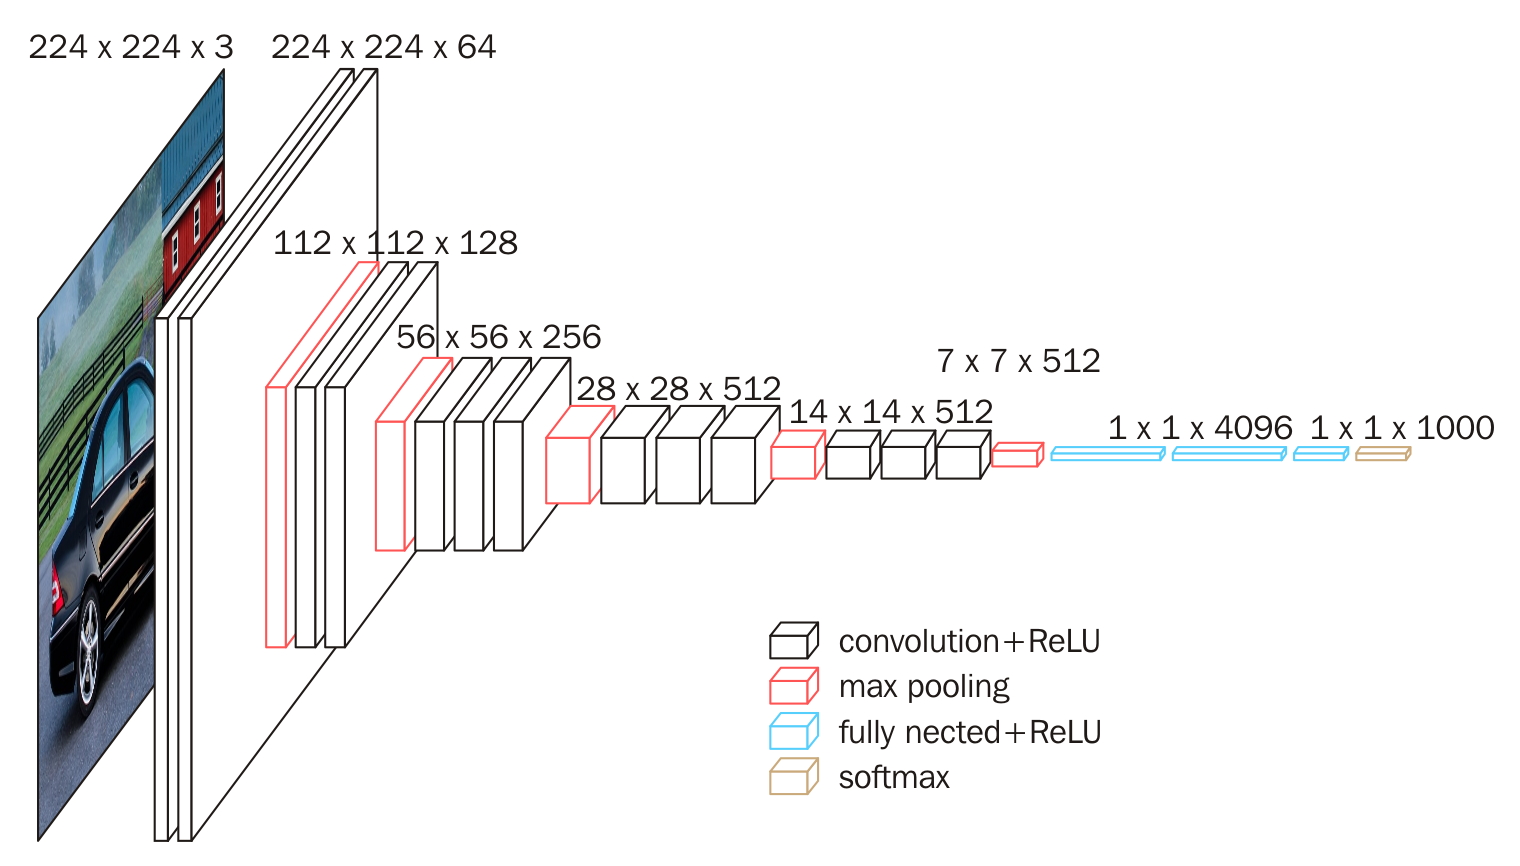
\includegraphics[width=1\textwidth]{vgg16.png}	%\vspace{-1.0em}
%    \caption{VGG-16,线性网络结构}
%    \label{fig:vgg16_} %\vspace{-0.8em}
%\end{figure}
%
%\subsection{残差网络与Shortcut连接}
%
%残差网络与Shortcut连接由ResNet \cite{he2016deep} 提出,使用Shortcut跳层连接,可以训练更深的神经网络。ResNet的结构如图~\ref{fig:resnet_}所示。ResNet(残差神经网络)是由微软研究院的何恺明等人提出的。残差神经网络的主要贡献是发现了“退化现象(Degradation)”,并针对退化现象发明了Shortcut连接,提出了带有旁路层的残差模块,帮助梯度在层与层之间能够更加容易的传递,解决了深度过大的神经网络训练困难的问题,使得神经网络的“深度”首次突破了100层,最大甚至可以超过1000层。
%
%\begin{figure}[]
%    \centering
%    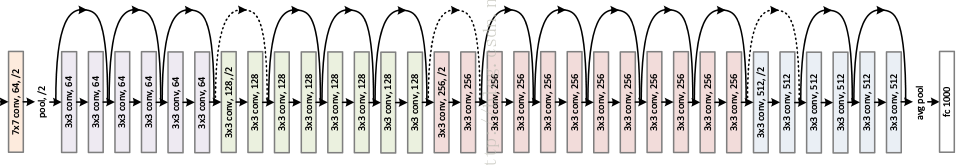
\includegraphics[width=1\textwidth]{resnet.png}	%\vspace{-1.0em}
%    \caption{ResNet,残差网络结构}
%    \label{fig:resnet_} %\vspace{-0.8em}
%\end{figure}
%
%ResNet使用两种不同的残差单元,如图~\ref{fig:residual}所示。左图对应的是浅层网络的残差结构,而右图对应的是深层网络的残差结构。对于Shortcut连接,当输入和输出维度一致时,可以直接将输入加到输出上。但是当维度不一致时,这就不能直接相加。有两种策略:(1)采用zero-padding增加维度,此时一般要先做一个downsamp,可以采用strde=2的pooling,这样不会增加参数;(2)一般采用1x1的卷积(projection shortcut),这样会增加参数,也会增加计算量。短路连接除了直接使用恒等映射,也可以采用1x1卷积。
%
%\begin{figure}[]
%    \centering
%    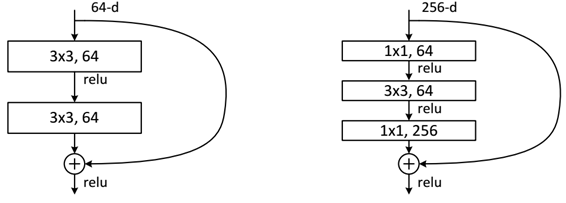
\includegraphics[width=1\textwidth]{residual.png}	%\vspace{-1.0em}
%    \caption{两种的残差结构}
%    \label{fig:residual} %\vspace{-0.8em}
%\end{figure}
%
%
%\subsection{多分支inception模块}
%
%GoogleNet使用inception模块作为其卷积的基本单元,inception模块是一种多分支和多尺度的卷积核拼接而成。如图~\ref{fig:googlenet_}所示,GoogleNet即Inception-V1,它以inception单元为基本结构,具有9个inception模块,每个inception模块由四个分支组成,分别是1×1、3×3、5×5卷积和down-sampling,具有多尺度感受野。inception结构的主要贡献有两个:一是使用1x1的卷积来进行升降维;二是使用多尺度的卷积核进行特征提取。训练时使用两个辅助损耗层从中间层注入Loss,防止梯度消失,而在推理时,删除辅助层。
%
%\begin{figure}[]
%    \centering
%    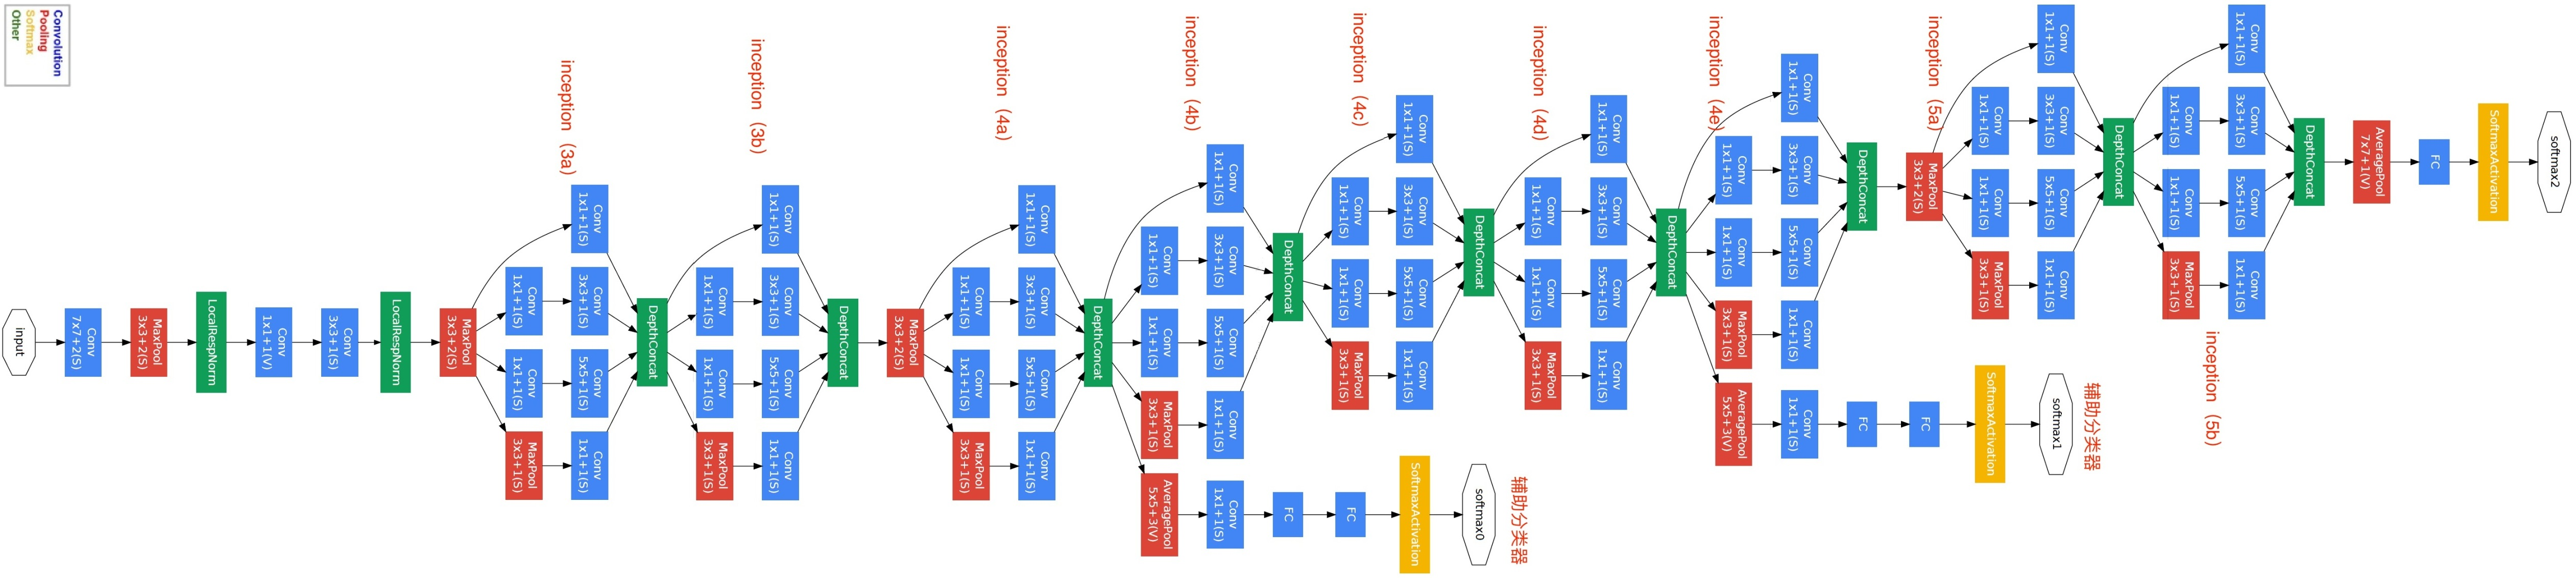
\includegraphics[width=1\textwidth]{googlenet.jpg}	%\vspace{-1.0em}
%    \caption{GoogleNet,多分支inception模块}
%    \label{fig:googlenet_} %\vspace{-0.8em}
%\end{figure}
%
%残差结构经过发展,有多种变形,但其主要思想就是通过在多分支上进行多尺度的卷积运算,在多个感受野上进行特征提取,为了减少计算量,使用两个3*3卷积代替5*5,使用1*7和7*1卷积代替7*7卷积。
%
%\begin{figure}[]
%    \centering
%    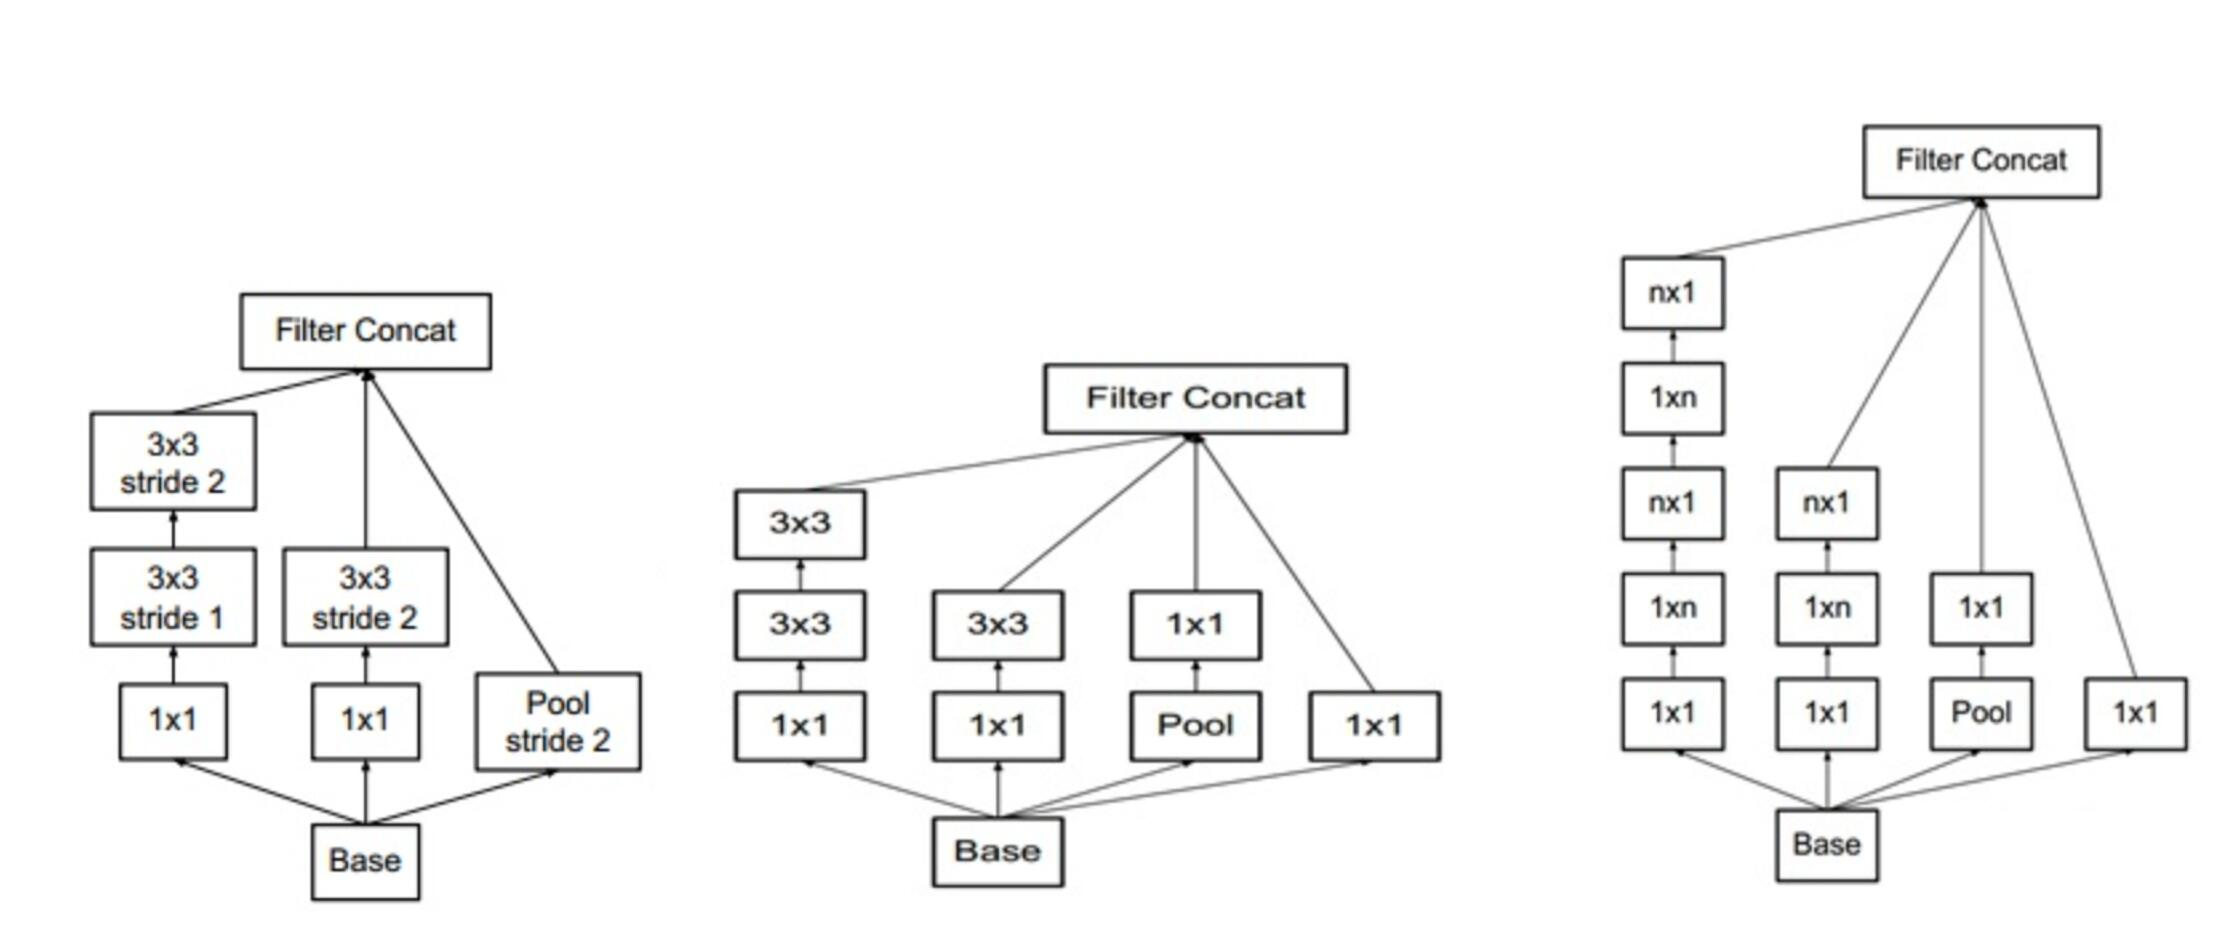
\includegraphics[width=1\textwidth]{inception.jpg}	%\vspace{-1.0em}
%    \caption{3种的残差结构}
%    \label{fig:inception} %\vspace{-0.8em}
%\end{figure}
%
%\subsection{线性网络与多分支网络对比}
%
%多分支网络结构如,残差模块通过shortcut快捷连接,直接将训练损失回传,避免了深层神经网络的退化问题,可以训练更深的网络;inception模块利用多分支卷积,通过合并多个感受野下的特征使得网络训练性能更好。它们都能提升网络参数的表达能力,对与网络训练是有意义的。但是,相比于单路结构,多分支结构对内存不友好,同时不利于并行化,并不能完全利用计算和内存资源。如图~\ref{fig:plain_res}所示,具有分支的结构会保存之前计算的特征图,在add或cat之前都需要常驻内存,对内存不友好。他们的优缺点如表\ref{tab:plain_res}所示,可以看到,多分支网络训练友好部署不友好,线性网络则恰好相反。
%
%\begin{figure}[]
%    \centering
%    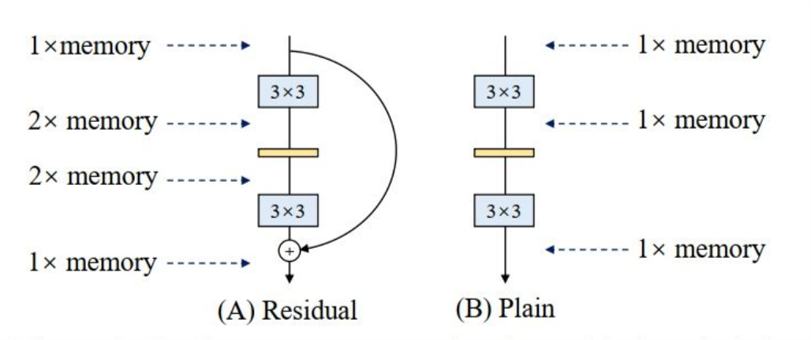
\includegraphics[width=1\textwidth]{plain_res.png}	%\vspace{-1.0em}
%    \caption{残差结构与线性网络内存使用对比}
%    \label{fig:plain_res} %\vspace{-0.8em}
%\end{figure}
%
%\begin{table}[]
%    \centering
%    \caption{线性网络与多分支网络优缺点}
%    \label{tab:plain_res} %\vspace{-0.8em}
%    \begin{tabular}{lll}
%    \hline
%    网络类型  & 优点                                                              & 缺点                                                      \\ \hline
%    线性网络  & \begin{tabular}[c]{@{}l@{}}并行度高\\ 内存效率高\\ 推理速度更快\end{tabular}   & \begin{tabular}[c]{@{}l@{}}不利于反向传播\\ 训练不友好\end{tabular} \\ \hline
%    多分支网络 & \begin{tabular}[c]{@{}l@{}}利于反向传播\\ 多尺度感受野\\ 参数效率高\end{tabular} & \begin{tabular}[c]{@{}l@{}}不利于并行\\ 内存效率低\end{tabular}   \\ \hline
%    \end{tabular}
%\end{table}
%
%\section{基于重参数化的残差模块融合}
%
%相比于各种多分支架构(如ResNet,Inception,DenseNet,各种NAS架构等),近年来VGG式的线性网络模型鲜有关注,主要自然是因为性能差。例如,有研究认为,ResNet性能好的一种解释是ResNet的分支结构(Shortcut)产生了一个大量子模型的隐式集成(因为每遇到一次分支,总的路径就变成两倍),单路架构显然不具备这种特点。既然多分支架构是对训练有益的,而我们想要部署的模型是单路架构,我们针对多分支网络中的典型网络模型ResNet提出一种解耦训练时和推理时的方法,将网络模型的训练和部署区分,流程如下:
%
%\begin{itemize}
%    %\vspace{-1em}
%    \item[1)] 训练ResNet网络模型
%    \item[2)] 将残差模块进行分支融合,去除Shortcut连接,等价转换为单个卷积核
%    \item[3)] 部署融合后模型
%\end{itemize}
%
%这样就可以同时利用残差结构训练时的优势(性能高)和线性模型推理时的好处(速度快、省内存)。这里的关键显然在如何将ResNet的残差模块进行处理和融合。
%
%为了能够顺利的融合残差模块,我们需要对残差模块进行一定修改。如图~\ref{fig:bbres_merge}和图~\ref{fig:blres_merge}所示,在训练时,确保能够在训练之后通过代数运算合并卷积核,我们将残差连接中的非线性层去掉,这是我们对ResNet的残差结构唯一的修改,基本不影响ResNet模型精度。但是去掉非线性层后,相互连接的卷积层就能够进行纵向融合成为一个卷积核,如图~\ref{fig:bbres_merge}所示,对于包含两个 3x3 卷积核的BasicBlock残差模块,去掉非线性层之后能够将整个残差模块融合为一个 5x5 的卷积核,虽然一个 5x5 的卷积核参数量比两个 3x3 卷积核稍大,但是在实际运行时其速度更快,且去除了分支结构,内存消耗更少。对于Bottleneck残差模块的融合如图~\ref{fig:blres_merge}所示则更为划算,融合之后的卷积核仍为 3x3 的卷积核。
%
%\begin{figure}[]
%    \centering
%    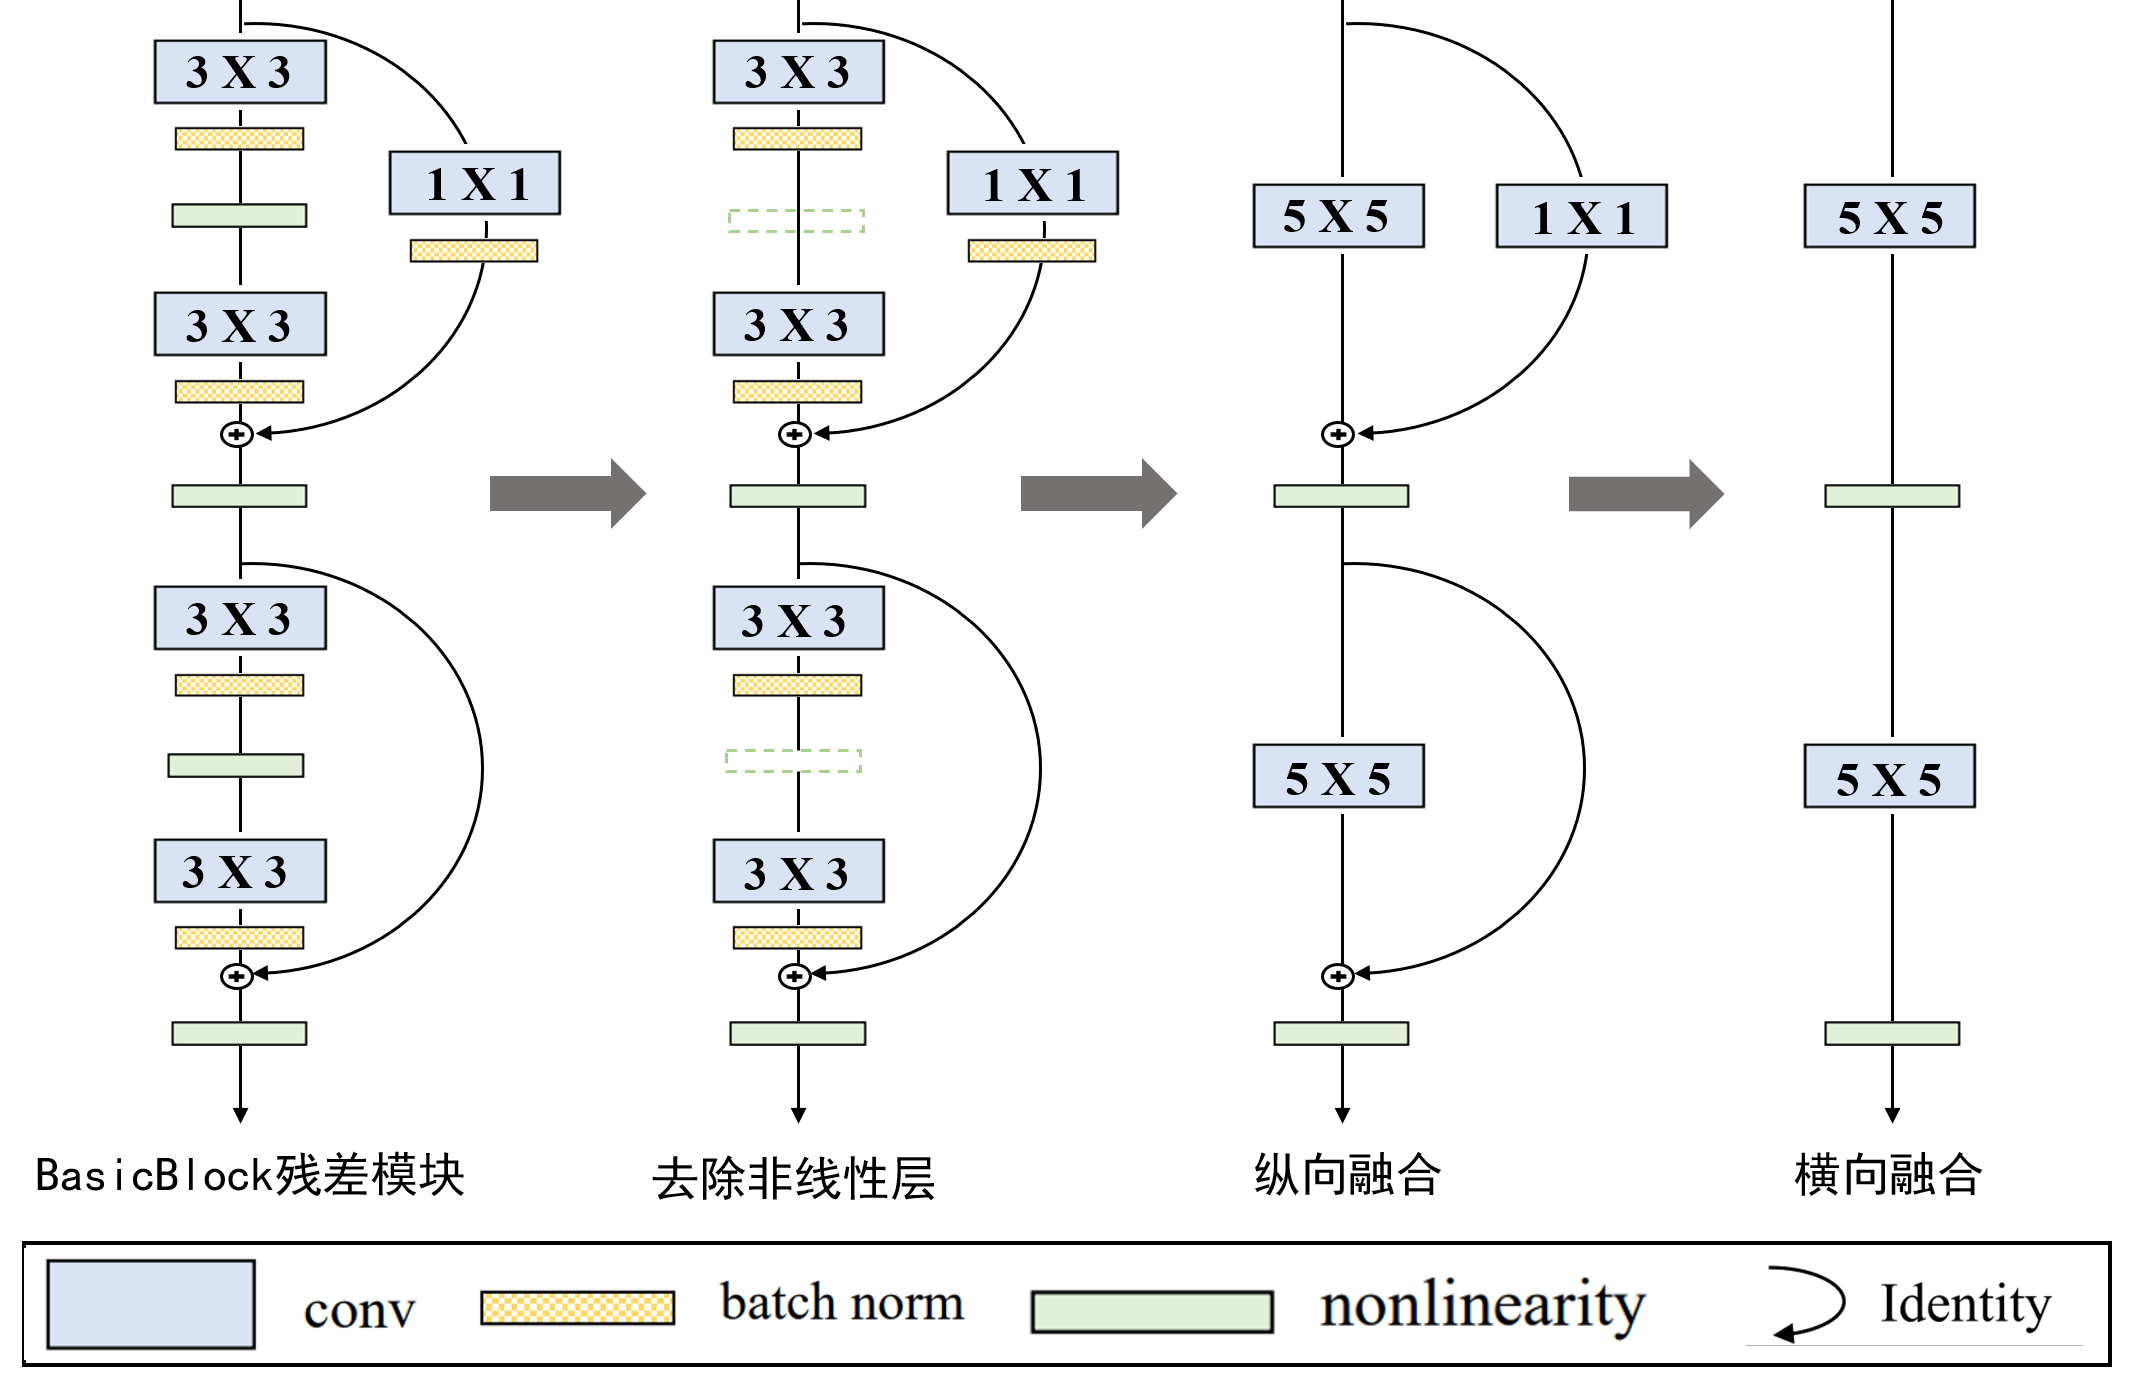
\includegraphics[width=1\textwidth]{bbres_merge.png}	%\vspace{-1.0em}
%    \caption{BasicBlock残差结构融合示意图}
%    \label{fig:bbres_merge} %\vspace{-0.8em}
%\end{figure}
%
%\begin{figure}[]
%    \centering
%    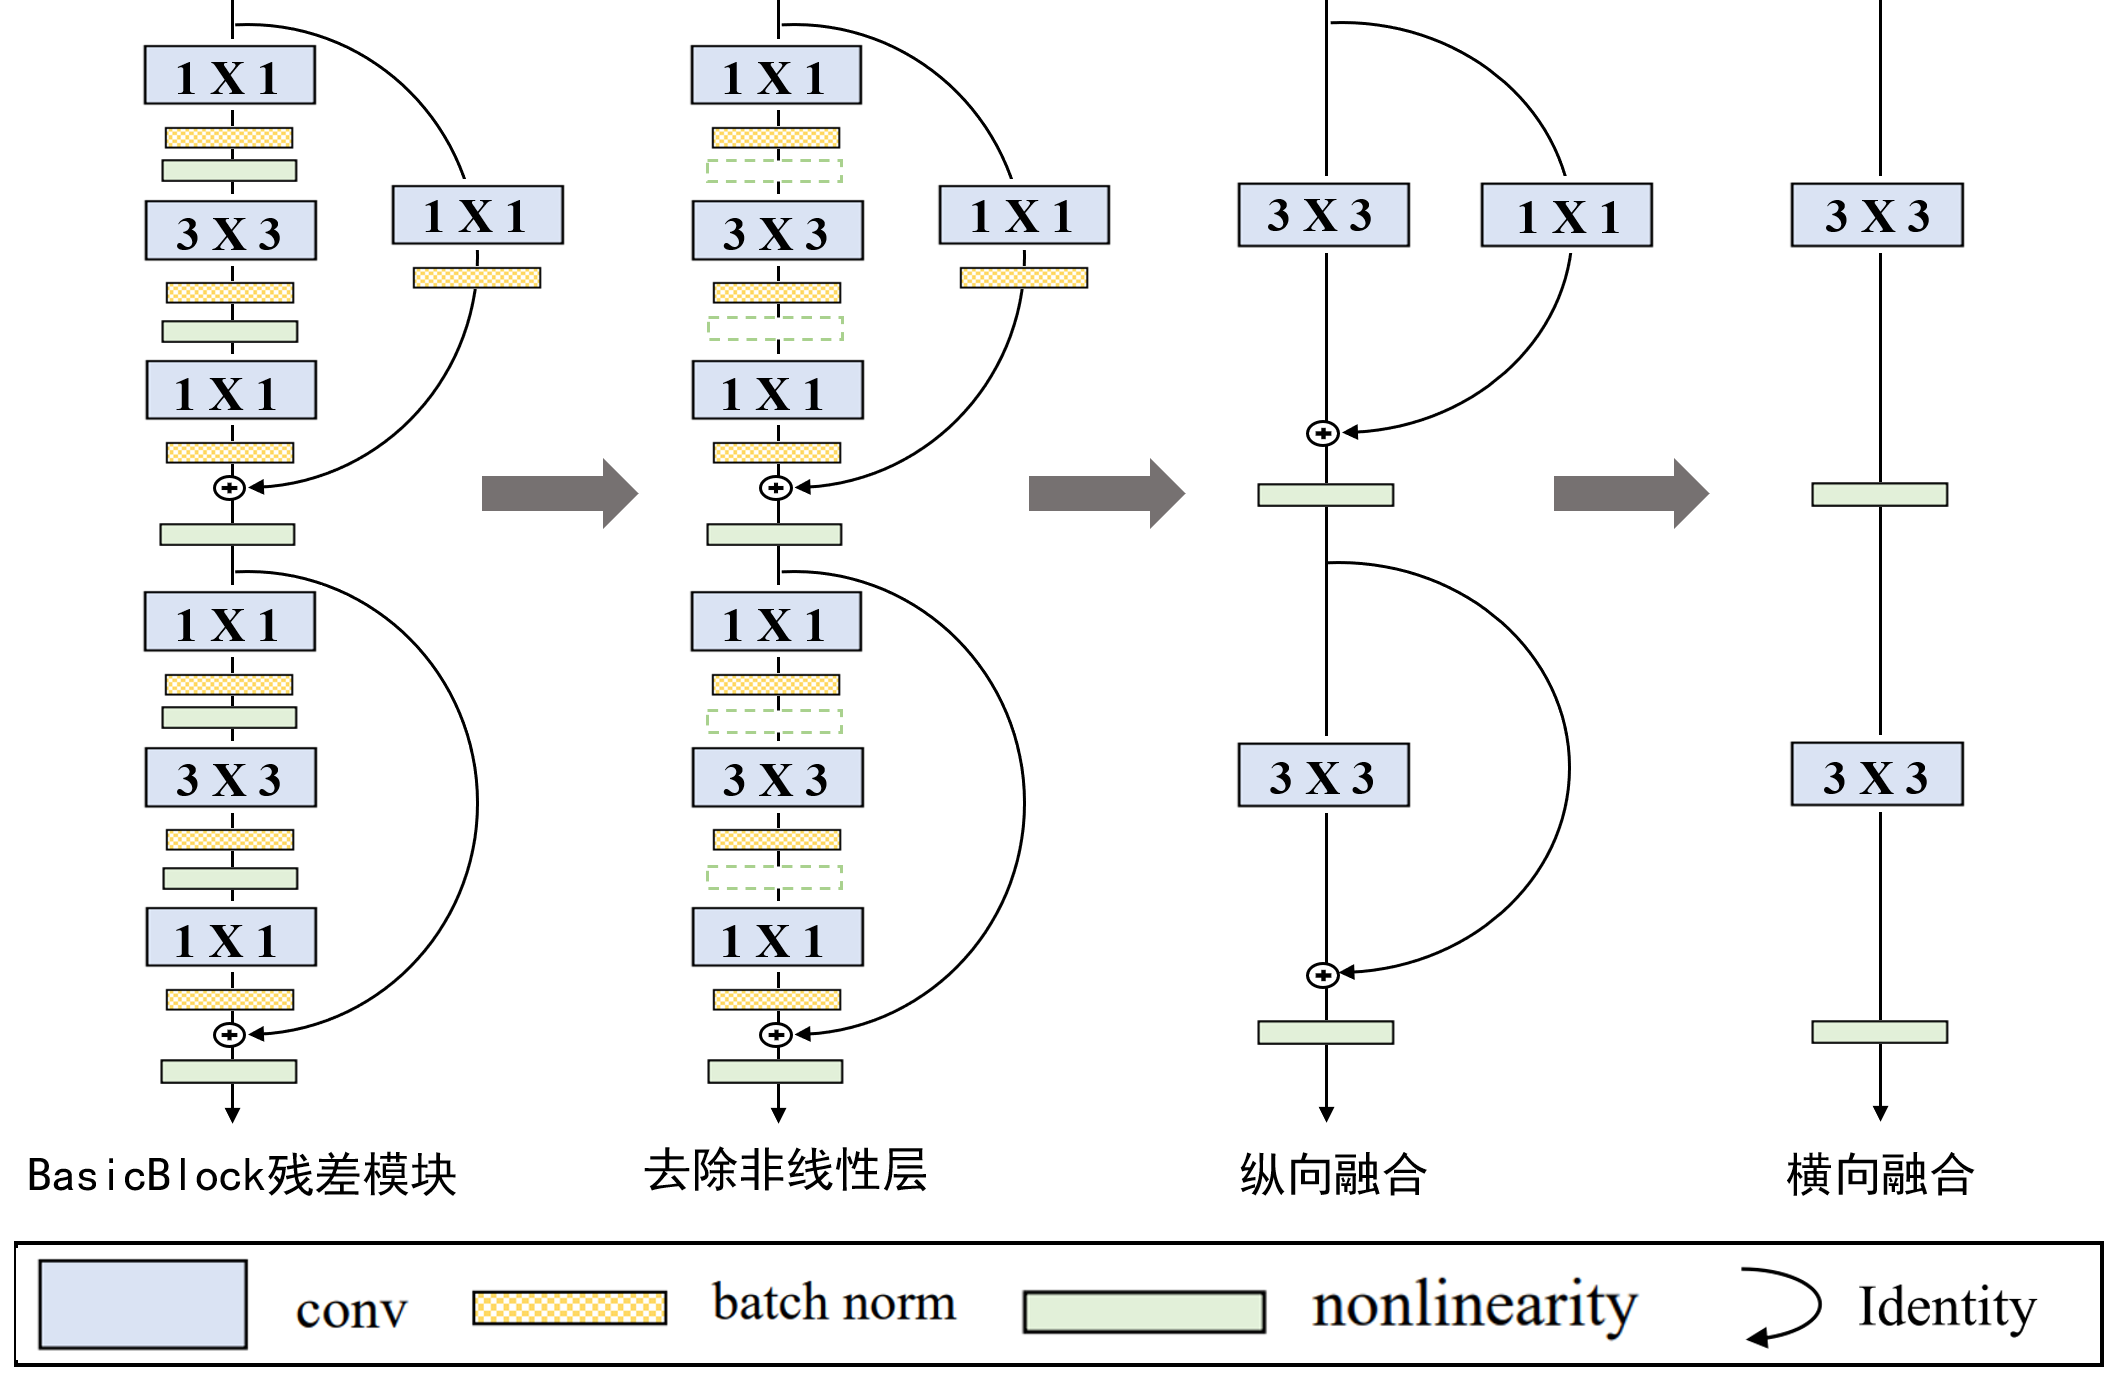
\includegraphics[width=1\textwidth]{blres_merge.png}	%\vspace{-1.0em}
%    \caption{Bottleneck残差结构融合示意图}
%    \label{fig:blres_merge} %\vspace{-0.8em}
%\end{figure}
%
%我们知道,不包含非线性层的卷积网络模块可以等价为一个线性函数,因此可以一步一步将其进行等价转换和等价合并。下面将具体描述残差网络的融合原理和融合方法,包括:
%\begin{itemize}
%    \item[1)] 卷积层和批归一化层融合
%    \item[2)] 卷积层纵向融合
%    \item[3)] 卷积层横向融合  
%\end{itemize}
%
%\subsection{卷积层和批归一化层合并}
%
%卷积层 (Conv层) 和批归一化层 (BN层) 很容易进行合并为一个卷积层,这是在部署时进行计算图优化的一个常用手段,通过合并 Conv + BN 层,可以减少网络层数,提升网络性能。其融合原理如下:
%
%卷积层公式为: 
%\begin{equation}
%    Conv(X) = WX + b
%\end{equation}
%BN层公式为:
%\begin{equation}
%    BN(X) = \gamma * \frac{-mean}{\sqrt{var}} + \beta
%\end{equation}    
%带入有: 
%\begin{equation}
%    \begin{aligned}
%        BN(Conv(X)) &= \gamma * \frac{WX + b - mean}{\sqrt{var}} + \beta \\
%                    &= \frac{\gamma * WX}{\sqrt{var}} + \frac{\gamma * (b - mean)}{\sqrt{var}} + \beta
%    \end{aligned}
%\end{equation}
%令:   
%\begin{equation}
%    \begin{aligned}
%        &Conv_{fused} = BN(Conv(x)) \\
%        &W_{fused} = \frac{\gamma * WX}{\sqrt{var}}     \\
%        &B_{fused} = \frac{\gamma * (b - mean)}{\sqrt{var}} + \beta \\
%    \end{aligned}
%\end{equation}
%则: 
%\begin{equation}
%    \begin{aligned}
%        Conv_{fused}(X) &= BN(Conv(X)) \\
%                        &= W_{fused}X + B_{fused}
%    \end{aligned}
%\end{equation}
%
%融合之后,新的卷积层的权重(weight)为 $W_{fused}$,其偏置(bias) 为 $B_{fused}$。
%
%Conv层与BN层融合代码如下:
%
%\lstinline[style = python]|Conv层与BN层融合|
%\begin{lstlisting}[style = python]
%    def merge_bn(conv: nn.Conv2d, bn: nn.Conv2d):
%        w, b = conv.weight.data, conv.bias.data
%        gamma = bn.weight.data
%        running_mean = bn.running_mean
%        running_var = bn.running_var
%        eps = bn.eps
%        std = (running_var + eps).sqrt()
%
%        w = conv[0].weight.data * ((gamma / std).reshape(-1, 1, 1, 1))
%        b = conv[1].bias.data - running_mean * gamma / std
%
%        return w, b
%\end{lstlisting}
%
%\subsection{卷积层纵向融合}
%
%直接的卷积层由于中间没有非线性层,其公式可表示为:
%\begin{equation}
%    \begin{aligned}
%        Conv_2(Conv_1(X)) &= W_2(W_1X+b_1) + b_2 \\
%                          &= W_2W_1X + W_2b_1 + b_2 \\
%                          &= (W_2W_1)X + (W_2b_1 + b_2)
%    \end{aligned}
%\end{equation} 
%令:
%\begin{equation}
%    \begin{aligned}
%        &Conv_{fused}(X) = Conv_2(Conv_1(X)) \\
%        &W_{fused} = (W_2W_1) \\
%        &b_{fused} = (W_2b_1 + b_2)
%\end{aligned}
%\end{equation}  
%则:
%\begin{equation}
%    \begin{aligned}
%        Conv_{fused} &= Conv_2(Conv_1(X)) \\
%                     &= (W_2W_1)X + (W_2b_1 + b_2) \\
%                     &= W_{fused} + b_{fused}
%    \end{aligned}
%\end{equation} 
%
%融合之后,新的卷积层的权重(weight)为 $W_{fused}$,其偏置(bias) 为 $B_{fused}$。
%为了详细说明,假设输入特征图特征图尺寸为[1, 2, 3, 3],连续经过一个 3x3 卷积层和 1x1 卷积层,输出特征图为[1, 2, 1, 1],如图~\ref{fig:merge31}所示,为连续3x3 卷积层和 1x1 卷积层的计算过程,由于 1x1 卷积比较特殊(非1x1卷积核融合计算稍显复杂,融合后的卷积核会增大,示例使用比较简单的包含1x1卷积的融合),此时可以看做由 1x1 卷积核先对 3x3卷积核参数做卷积运算,将所得的的参数当做新卷积层参数,再对输入进行卷积。Conv3x3与Conv1x1纵向融合代码如下:
%
%\lstinline[style = python]|Conv3x3与Conv1x1纵向融合|
%\begin{lstlisting}[style = python]
%    # 先Conv3x3再Conv1x1
%    def merge_3_1(conv3: nn.Conv2d, conv1: nn.Conv2d):
%        k1, k3 = conv1.weight.data, conv3.weight.data
%        b1, b3 = conv1.bias.data, conv3.bias.data
%
%        print(k1.shape, k3.shape)
%        k = F.conv2d(k3.permute(1, 0, 2, 3), k1).permute(1, 0, 2, 3)
%        b = (k1 * b3.reshape(1, -1, 1, 1)).sum((1, 2, 3)) + b1
%        print(b.shape)
%        return k, b
%
%    # 先Conv1x1再Conv3x3
%    def merge_1_3(conv1: nn.Conv2d, conv3: nn.Conv2d):
%        k1, k3 = conv1.weight.data, conv3.weight.data
%        b1, b3 = conv1.bias.data, conv3.bias.data
%
%        k = F.conv2d(k3, k1.permute(1, 0, 2, 3))
%        b = (k3 * b1.reshape(1, -1, 1, 1)).sum((1, 2, 3)) + b3
%        print(b.shape)
%        return k, b
%\end{lstlisting}
%
%\begin{figure}[]
%    \centering
%    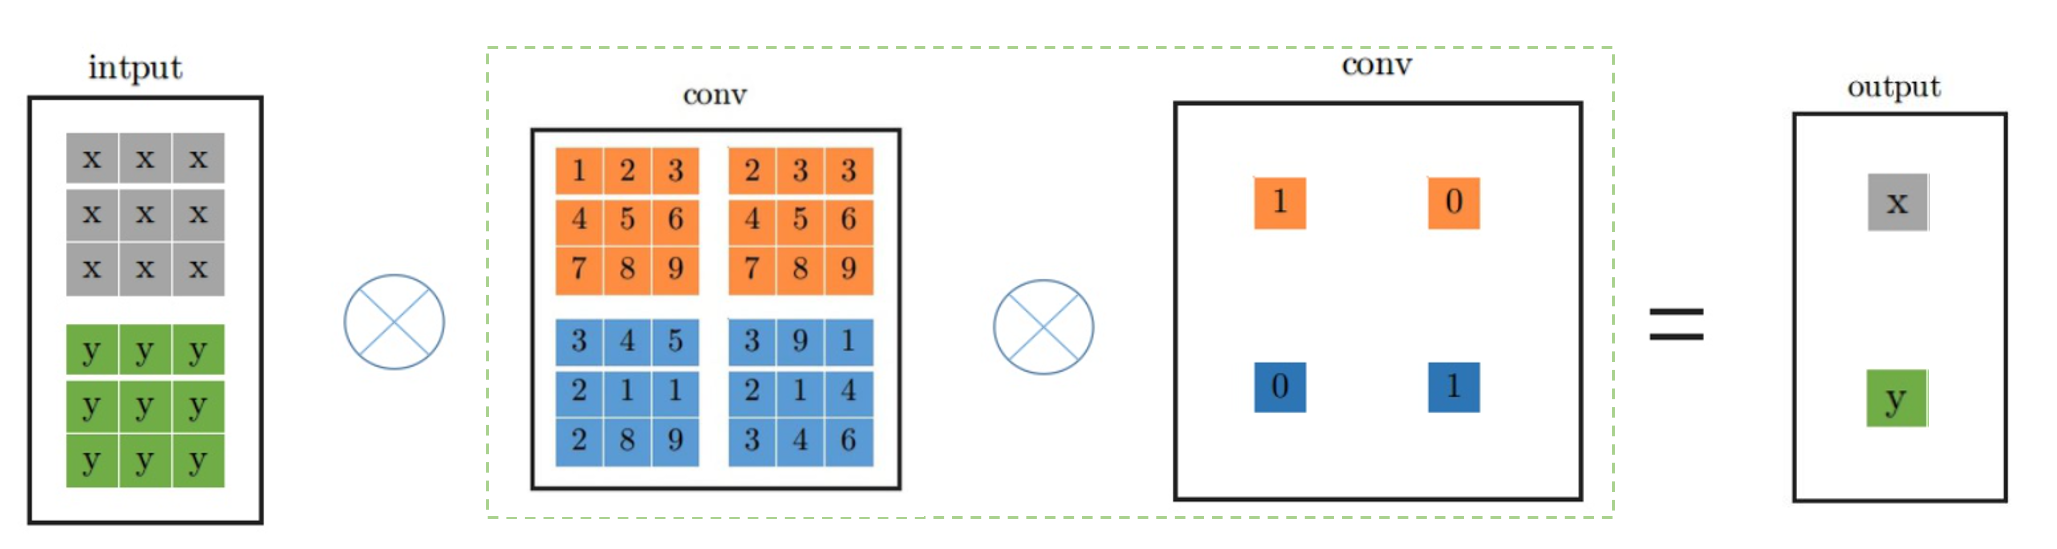
\includegraphics[width=1\textwidth]{merge31.png}	%\vspace{-1.0em}
%    \caption{Conv3*3与Conv1*1纵向融合}
%    \label{fig:merge31} %\vspace{-0.8em}
%\end{figure}
%
%\subsection{卷积层横向融合}
%
%在残差结构中,使用逐元素相加的方式合并不同的分支,对于特征图,要求不同分支的特征图维度完全一样,对于卷积参数融合,要求不同分支的卷积核参数维度完全一样,因此,对于 1x1 卷积和 Identity连接需要特殊处理。
%
%\begin{itemize}
%    %\vspace{-1em}
%    \item[1)] 1x1卷积等价扩充: 
%    
%    对于卷积操作,小卷积核可以看做是大卷积核的一种特例,小卷积核可以用大卷积核来进行描述,如图~\ref{fig:pad13}所示,1x1卷积核可以进行补0,将其扩充为3x3卷积核,由3x3卷积核表示。
%
%    \begin{figure}[]
%        \centering
%        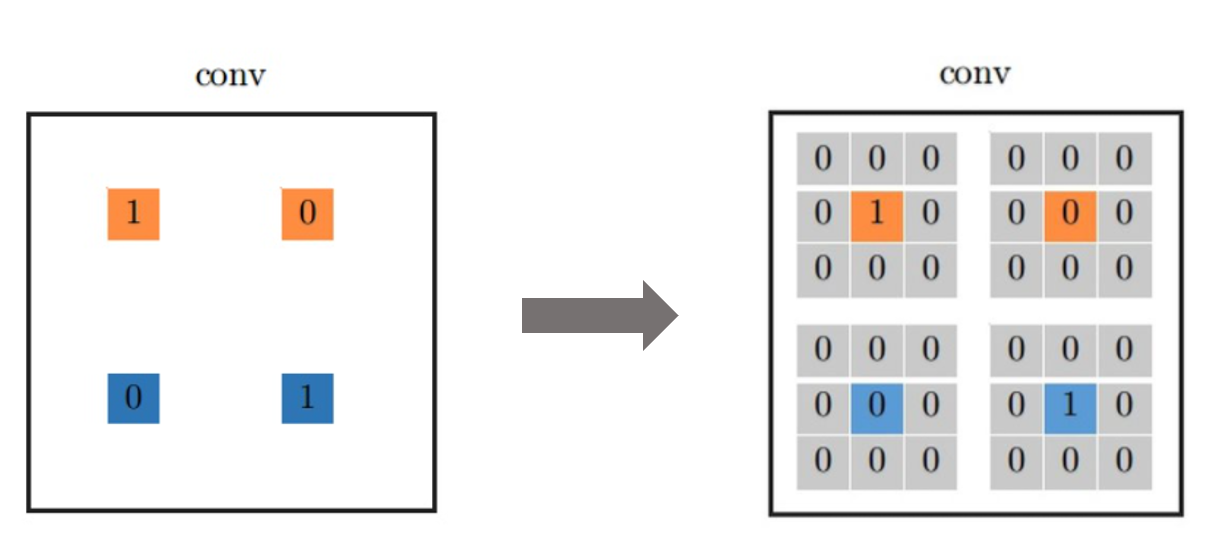
\includegraphics[width=0.8\textwidth]{kernel1_3.png}	%\vspace{-1.0em}
%        \caption{Conv1*1卷积核等价扩充表示}
%        \label{fig:pad13} %\vspace{-0.8em}
%    \end{figure}
%
%    \item [2)] Identity层等价卷积核:  
%    
%    identity层就是输入等于输出,即input中每个通道每个元素直接输出到output中对应的通道,即相当于值为1的深度可分离卷积,使用普通卷积表示为单位矩阵,因此,identity可以等效成如下图~\ref{fig:fuse31-4}的Conv1*1的卷积形式。我们进一步可以将identity -> Conv1*1 -> Conv3*3的形式,如下图~\ref{fig:fuse31-5}所示。
%
%    \begin{figure}[]
%        \centering
%        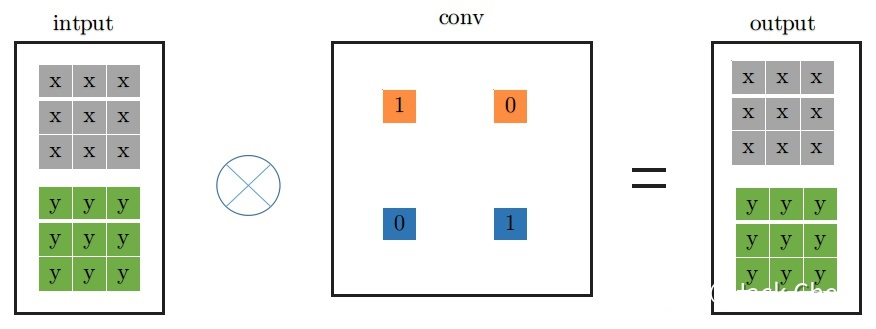
\includegraphics[width=0.8\textwidth]{fuse31_4.jpg}	%\vspace{-1.0em}
%        \caption{identity层的Conv1*1表示}
%        \label{fig:fuse31-4} %\vspace{-0.8em}
%    \end{figure}
%    
%    \begin{figure}[]
%        \centering
%        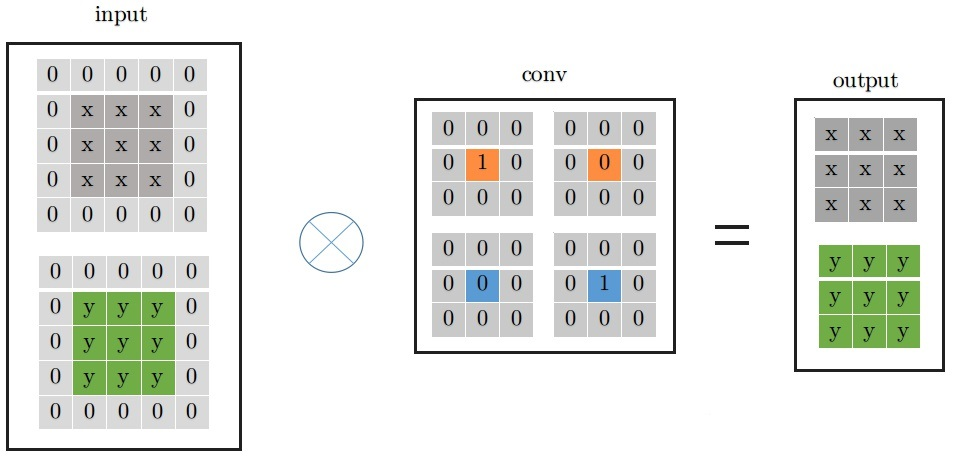
\includegraphics[width=0.8\textwidth]{fuse31_5.jpg}	%\vspace{-1.0em}
%        \caption{identity层的Conv3*3表示}
%        \label{fig:fuse31-5} %\vspace{-0.8em}
%    \end{figure}
%
%\end{itemize}
%
%为了详细说明,假设输入特征图特征图尺寸为(1, 2, 3, 3),输出特征图尺寸与输入特征图尺寸相同,且stride=1,如图~\ref{fig:fuse31-1},展示是Conv3*3的卷及过程:
%
%Conv3*3卷积由上图所示,首先将特征图进行 $pad=kernel_size//2$,然后从上图左上角红色为止做卷积运算,最终得到右边output输出。如图~\ref{fig:fuse31-2}是Conv1*1卷积过程:
%
%同理,Conv1*1跟Conv3*3卷积过程一样,从上图中左边input中红色位置开始进行卷积,得到右边的输出,观察Conv1*1和Conv3*3的卷积过程,从红色起点位置开始,走过相同的计算路径,因此,将Conv1*1跟Conv3*3进行融合,只需要将Conv1*1卷积核padding成Conv3*3的形式,然后于Conv3*3相加,再与特征图做卷积(这里依据卷积的可加性原理)即可,也就是Conv1*1的卷积过程变成如下图~\ref{fig:fuse31-3}形式:
%
%\begin{figure}[]
%    \centering
%    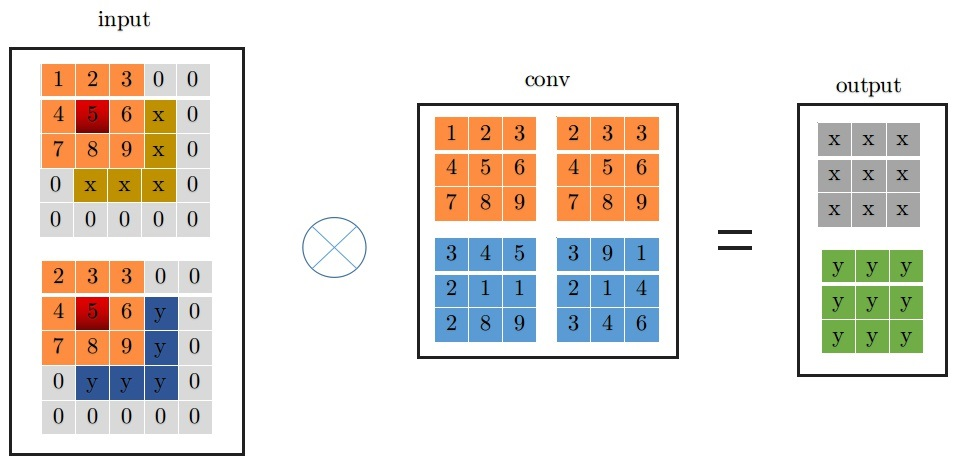
\includegraphics[width=0.8\textwidth]{fuse31_1.jpg}	%\vspace{-1.0em}
%    \caption{Conv3*3卷积运算}
%    \label{fig:fuse31-1} %\vspace{-0.8em}
%\end{figure}
%
%\begin{figure}[]
%    \centering
%    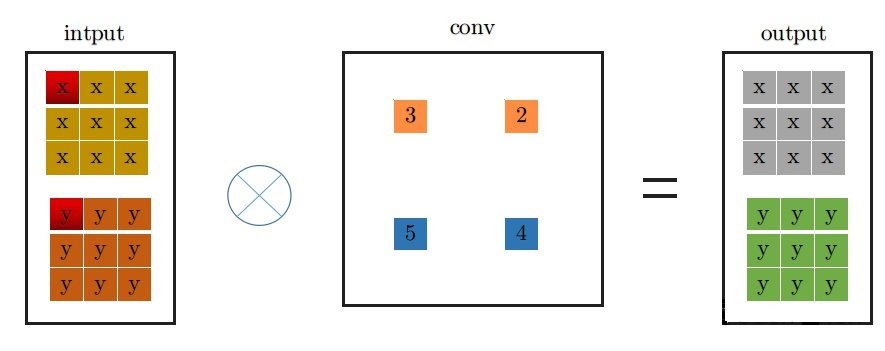
\includegraphics[width=0.8\textwidth]{fuse31_2.jpg}	%\vspace{-1.0em}
%    \caption{Conv1*1卷积运算}
%    \label{fig:fuse31-2} %\vspace{-0.8em}
%\end{figure}
%
%\begin{figure}[]
%    \centering
%    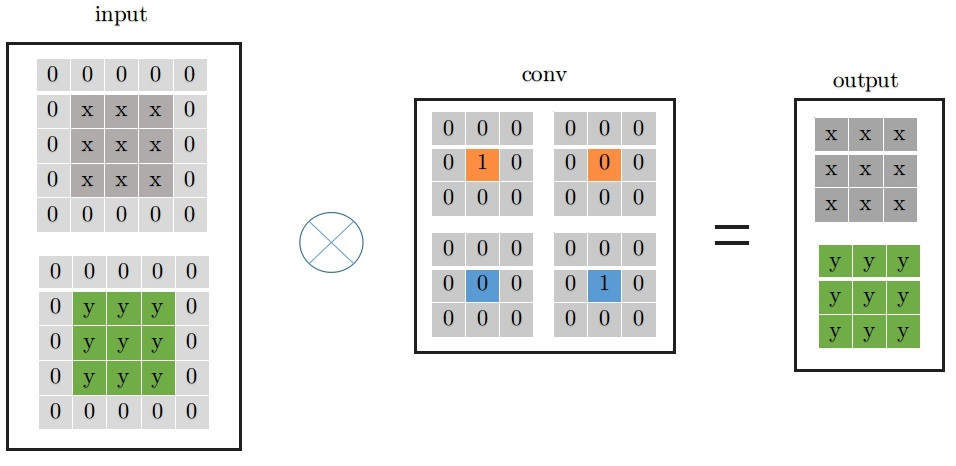
\includegraphics[width=0.8\textwidth]{fuse31_3.jpg}	%\vspace{-1.0em}
%    \caption{Conv3*3 和 Conv1*1合并步骤3}
%    \label{fig:fuse31-3} %\vspace{-0.8em}
%\end{figure}
%
%在将分支转化为同等的卷积结构后,如图~\ref{fig:fuseall}将Conv1*1与identity都表示为Conv3*3形式,吸收BN层,然后线性可加。
%
%\begin{figure}[]
%    \centering
%    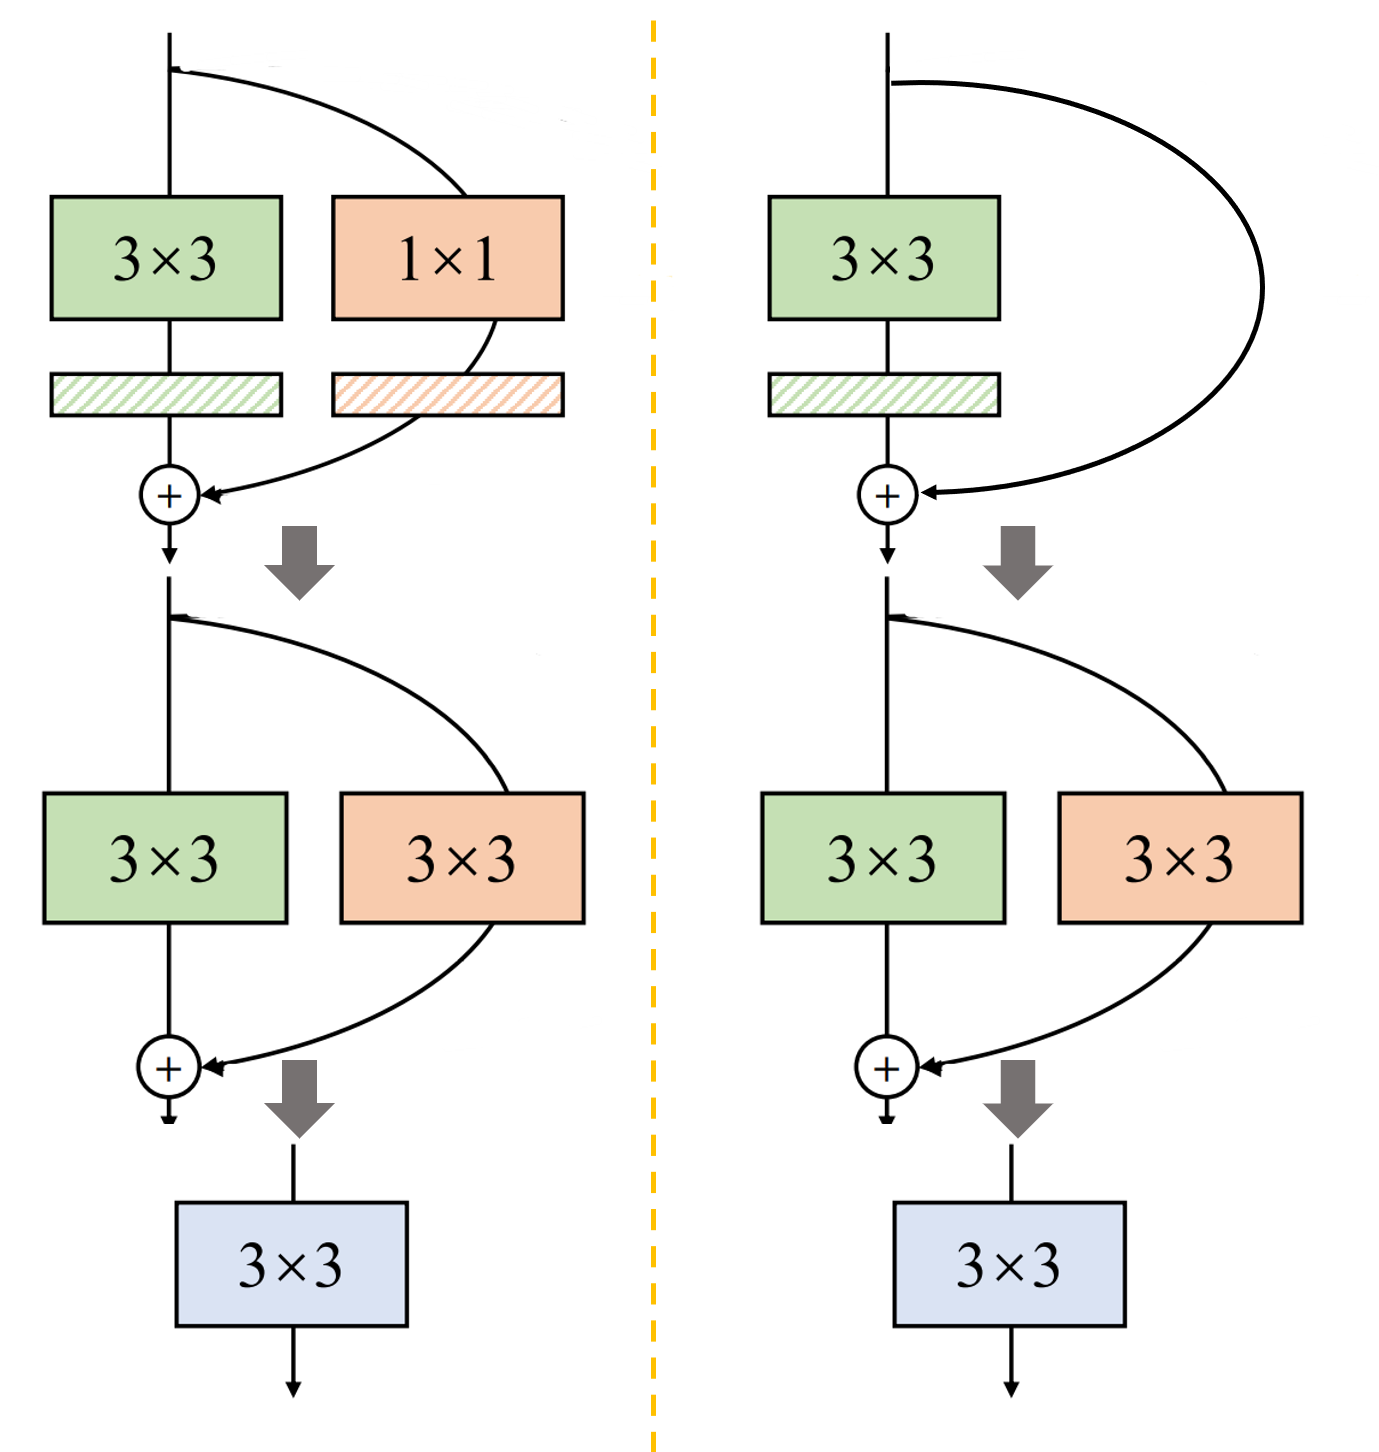
\includegraphics[width=0.8\textwidth]{fuseall.png}	%\vspace{-1.0em}
%    \caption{残差模块横向融合}
%    \label{fig:fuseall} %\vspace{-0.8em}
%\end{figure}
%
%\section{残差模块融合收益分析与通道调整}
%
%通过移除残差模块中的非线性层,可以很容易的将其进行合并,但是直接合并而不经任何修改可能会导致参数量的剧增,并不能带来明显的收益。下面将对ResNet网络中的不同残差模块的融合收益进行分析,并根据结果调整残差模块的通道结构。
%
%\subsection{BasicBlock残差模块}
%
%BasicBlock残差模块由一个 Shortcut 残差连接与两个连续的 3x3 卷积核组成,但是如果遇到需要下采样的情况,
%
%\subsubsection{无下采样的BasicBlock残差模块}
%
%\subsection{Bottleneck残差模块}
%
%
%\section{实验结果与分析}
%
%在本节中,我们在算力较高搭载V100 GPU的服务器上和算力较低的嵌入式设备TX2上进行了部署推理实验,比较了融合分支后的网络模型对比原始ResNet的推理性能。同时也在Cifar100和ImageNet数据集上进行了训练,对比融合分支后的网络模型与原始ResNet的精度差异。
%
%\subsection{实验设置}
%
%实验使用简单数据增强后的Cifar100、ImageNet数据集,训练120个周期,推理批量尺寸(batchsize)为256,速度单位为示例/秒,服务器显卡为 NVIDIA V100,嵌入式设备为NVIDIA TX2,使用 TensorRT 作为测试的软件环境。在实验对比中,我们将所提出针对残差结构的分支融合方法应用于ResNet上,并与原始的ResNet在运行速度,模型精度,内存消耗量上进行了比较。
%
%\subsubsection{硬件平台说明}
%
%我们实验的训练服务器使用 Intel Xeon E5服务器,配有2张 NVIDIA V100 显卡,其具体配置如表~ref{tbb:server}所示。
%
%\begin{table}[]
%    \centering
%    \caption{训练服务器配置表}
%    \label{tab:server} %\vspace{-0.8em}
%    \begin{tabular}{|l|l|}
%    \hline
%    OS  & Ubuntu 16.04 Xenial                  \\ \hline
%    CPU & 2 * Intel Xeon E5-2620 v4 @ 32x 3GHz \\ \hline
%    GPU & 2 * Nvidia Tesla V100             \\ \hline
%    RAM & 256GB DDR4                           \\ \hline
%    \end{tabular}
%\end{table}
%
%在部署时还在嵌入式平台上进行测试,使用 Nvidia TX2 作为部署环境,其搭载四核ARM®Cortex®-A57 MPCore, 8GB 256位LPDDR4内存,操作系统为Ubuntu 18.04。其具体配置如表~\ref{tab:tx2}所示。
%
%\begin{table}[]
%    \centering
%    \caption{Nvidia TX2配置表}
%    \label{tab:tx2} %\vspace{-0.8em}
%    \begin{tabular}{|l|l|}
%    \hline
%    OS   & Ubuntu 18.04 bionic            \\ \hline
%    CPU  & HMP Dual Denver + Quad ARM A57 \\ \hline
%    GPU  & Nvidia Pascal 256 CUDA cores   \\ \hline
%    RAM  & 8GB 128-bit LPDDR4             \\ \hline
%    DISK & 32GB eMMC                      \\ \hline
%    \end{tabular}
%\end{table}
%
%\subsection{实验结果}
%
%表~\ref{tab:acc_result}为分别在Cifar100和ImageNet上的训练结果,本次测试将分支融合部署的ResNet18、ResNet34、ResNet50、ResNet101与其原始模型进行对比,实验表明,我们的分支融合方法在误差范围内对模型精度并不影响。
%
%\begin{table*}
%    \caption{ImageNet上训练结果对比}
%     \label{tab:acc_result}
%    \begin{floatrow}
%    \capbtabbox{
%        \begin{tabular}{lll}
%            \hline
%            模型                 & Top1准确率           \\ \hline
%            ResNet18            & 78.61           \\
%            \textbf{ResNet18*}  & \textbf{78.83}  \\ \hline
%            ResNet34            & 78.84           \\
%            \textbf{ResNet34*}  & \textbf{78.63}  \\ \hline
%            ResNet50            & 77.88           \\
%            \textbf{ResNet50*}  & \textbf{79.26}  \\ \hline
%            ResNet101           & 80.16           \\
%            \textbf{ResNet101*} & \textbf{80.87} \\ \hline
%            ResNet152           & 80.99           \\
%            \textbf{ResNet152*} & \textbf{80.34} \\ \hline
%        \end{tabular}
%    }{
%     \caption{Cifar100上训练结果对比}
%     \label{tab:acc_result_tb1}
%    }
%    \capbtabbox{
%        \begin{tabular}{lll}
%            \hline
%            模型                 & Top1准确率            \\ \hline
%            ResNet18            & 71.16           \\
%            \textbf{ResNet18*}  & \textbf{71.21}  \\ \hline
%            ResNet34            & 74.17           \\
%            \textbf{ResNet34*}  & \textbf{74.36}  \\ \hline
%            ResNet50            & 76.31            \\
%            \textbf{ResNet50*}  & \textbf{76.48}   \\ \hline
%            ResNet101           & 77.21            \\
%            \textbf{ResNet101*} & \textbf{77.28}  \\ \hline
%            ResNet101           & 77.78            \\
%            \textbf{ResNet101*} & \textbf{77.56}  \\ \hline
%        \end{tabular}
%    }{
%     \caption{ImageNet上训练结果对比}
%     \label{tab:acc_result_tb12}
%    }
%    \end{floatrow}
%\end{table*}
%
%表~\ref{tab:speed_result}为在服务器端与嵌入式端实际部署时的推理速度对比。本次测试将分支融合部署的ResNet18、ResNet34、ResNet50、ResNet101、ResNet152与其原始模型进行对比,实验表明,在公平的训练设定下,同精度的分支融合部署的模型在速度和内存占用方面显著优于原有模型,
%效果非常不错。
%
%\begin{table}[]
%    \centering
%    \caption{ImageNet上训练结果对比}
%    \label{tab:speed_result} %\vspace{-0.8em}
%    \begin{tabular}{lll}
%    \hline
%    模型                  & TX2 速度       & V100 速度                    \\ \hline
%    ResNet18            & 71.16          & 2442                          \\
%    \textbf{ResNet18*}  & \textbf{72.41} & \textbf{3256}                 \\ \hline
%    ResNet34            & 74.17          & 1419                          \\
%    \textbf{ResNet34*}  & \textbf{74.46} & \textbf{2339}                 \\ \hline
%    ResNet50            & 76.31          & 719                           \\
%    \textbf{ResNet50*}  & \textbf{77.78} & \textbf{792}                  \\ \hline
%    ResNet101           & 77.21          & 430                           \\
%    \textbf{ResNet101*} & \textbf{78.78} & \textbf{460}                  \\ \hline
%    \end{tabular}
%\end{table}
%
%\section{本章小结}
%
%考虑到模型训练时和部署时的注重点不同,借助重参数化的思想,本章提出了针对残差结构的分支融合方法,优化部署时残差网络模型推理效率和内存效率。通过去除残差结构中的非线性层,在部署前融合多分支结构,在不损失模型精度的前提下,去除模型分支结构同时减少模型层数,提高部署时内存效率和运行效率。首先,讨论了到线性网络结构和多分支网络结构各自的优点和局限性,其次通过微调ResNet网络结构,解耦网络的训练和部署,在训练时使用多分支残差网络结构,在部署时将其转化为线性网络结构,同时利用了线性网络和多分支网络的优点而规避它们的缺点,最终获得在速度和精度两方面的性能提升。



